\documentclass{article}
\usepackage{graphicx} % Required for 
\usepackage{natbib} % For bibliography
\usepackage{float} % Add this in your preamble


\title{paper collagen}
\author{robert.tavares}
\date{November 2023}

\begin{document}

\maketitle

\section{Introduction}

O colágeno tipo I é uma proteína abundante no corpo humano, de forma que compõe $90\%$ dele. Ele está presente na matriz extracelular bem como em estruturas como pele, osso, tendão e córnea \cite{RicoLlanos2021, Silver2018}.
\\

O colágeno tipo I é uma molécula composta por um tripla hélice de cadeias polipeptídicas(cadeias $\alpha$). Ele possui tamanhos típicos de $300$ nm de comprimento por $1,5$ nm de diâmetro e apresenta um formato tipo haste \cite{Gelse2003,Silver2018}. 
\\

As moléculas de colágeno tipo I possuem, intrisicamente, a informação necessária para se auto-organizar em estruturas mais complexas chamadas fibrilas. Esse processo, denominado fibrilo-gênese, ocorre o mediante a agregação de milhares dessas moléculas de forma escalonada por um período $D= 67$ nm, de modo que existem cinco posições possíveis para que ocorra a interação entre elas\cite{Zhu2018, KADLER1996}.  
\\

As fibrilas apresentam um formato alongado, com a sua região mais densa sendo a central e, consequentemente, as pontas afinadas\cite{Charvolin2019, KADLER1996}. As fibrilas apresentam comprimento típicos de $500 \mu m$ com $500 nm$ de diâmetro, além de serem constituídas por moléculas da ordem de $10^{7}$\cite{Parry1984}. 
\\


\section{Metodologia}

    Em nosso trabalho, nos desenvolvemos o estudo em duas etapas: Modelo para formação de fibrilas e Morfologia e 
    propriedades mecânicas das fibrilas.

    \subsection{Formação de fibrilas}

        Nos utilizamos um modelo baseado em DLA(difusion limited aggregation)\cite{Witten1983} em três dimensões para 
        simular a formação de fibrilas de colágeno. Nos consideramos as moléculas de colágeno como  sendo paralelepitedos 
        regulares de dimensções 1 x 18 x 1. Usando uma rede regular cúbica, nos definimos o centro como a origem e fixamos
        a primeira molécula do agregado, chamada de seed, em seguida, novas moléculas são lançadas de uma distância $R$ do 
        centro  do agregado e se difundem até encontrarem o agregado e serem capturadas ou atingirem 
        uma distância  $2R$ com relação ao centro, de modo que a simulação é reiniciada caso isso ocorra, esse processo está 
        esquematizado na Figura \ref{M1}. 

        \begin{figure}[H]
            \centering
            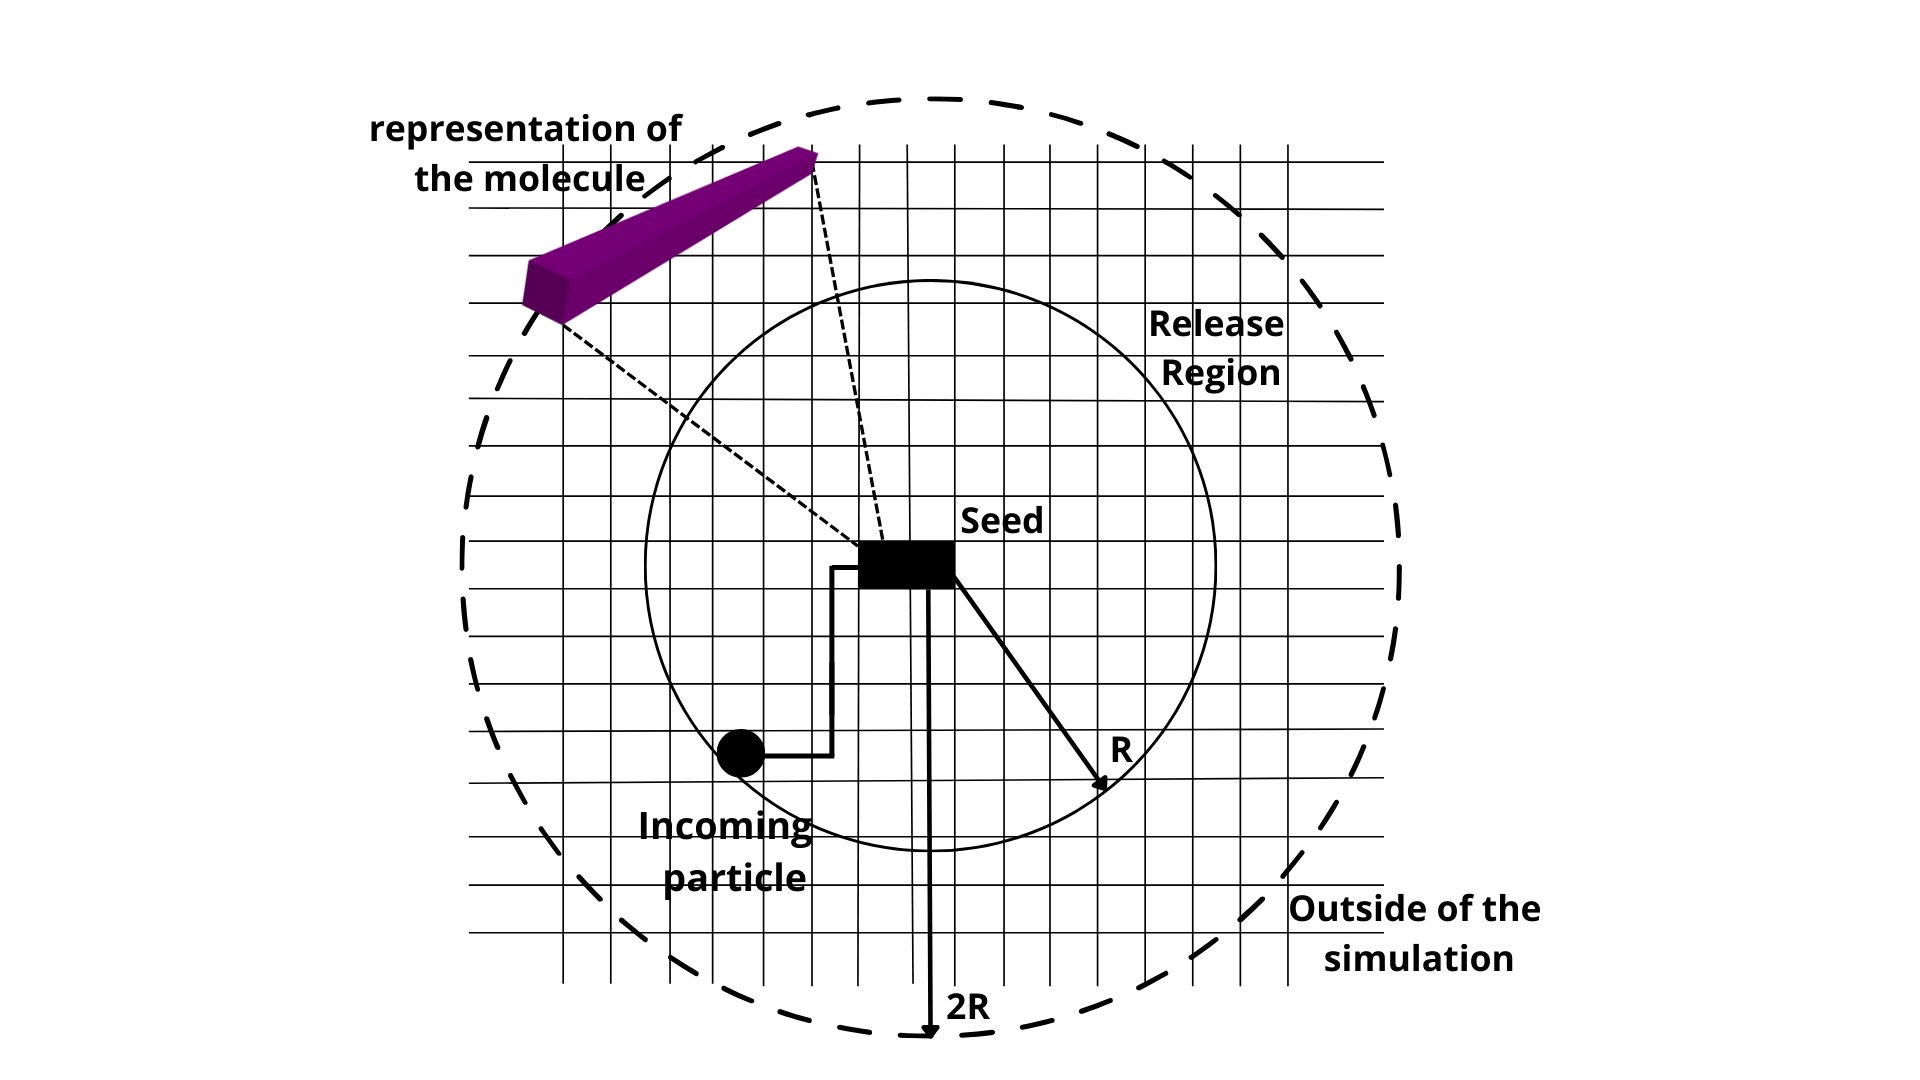
\includegraphics[width=\textwidth]{figures/DLA.png}
    
            \caption{.} 
    
            \label{M1}
        \end{figure}
    
        O processo de difusão dessas moléculas acontece mediante um random walk tridimensional.  As moléculas podem caminhar
        para os primeiros e os segundos vizinhos, no plano X-Z, no eixo Y, elas realizam movimento para frente e para tras. As moléculas 
        de colageno reais se agregam de forma lateral e em posições escalonadas com relação ao comprimento D = 67 nm. Dessa forma,
        ao atingir o agregado, a molécula é capturada apenas se ela estiver em uma posições especificas, multiplos de D = 4, com relação 
        a uma molécula pertencente ao agregado\cite{Parkinson1995}.  Dessa forma, visto o tamanho 18 da nossa representação,temos cinco 
        configurações possiveis para que uma molécula seja captura, na Figura \ref{M2} podemos ver cada posição possivel. 

        \begin{figure}[H]
            \centering
            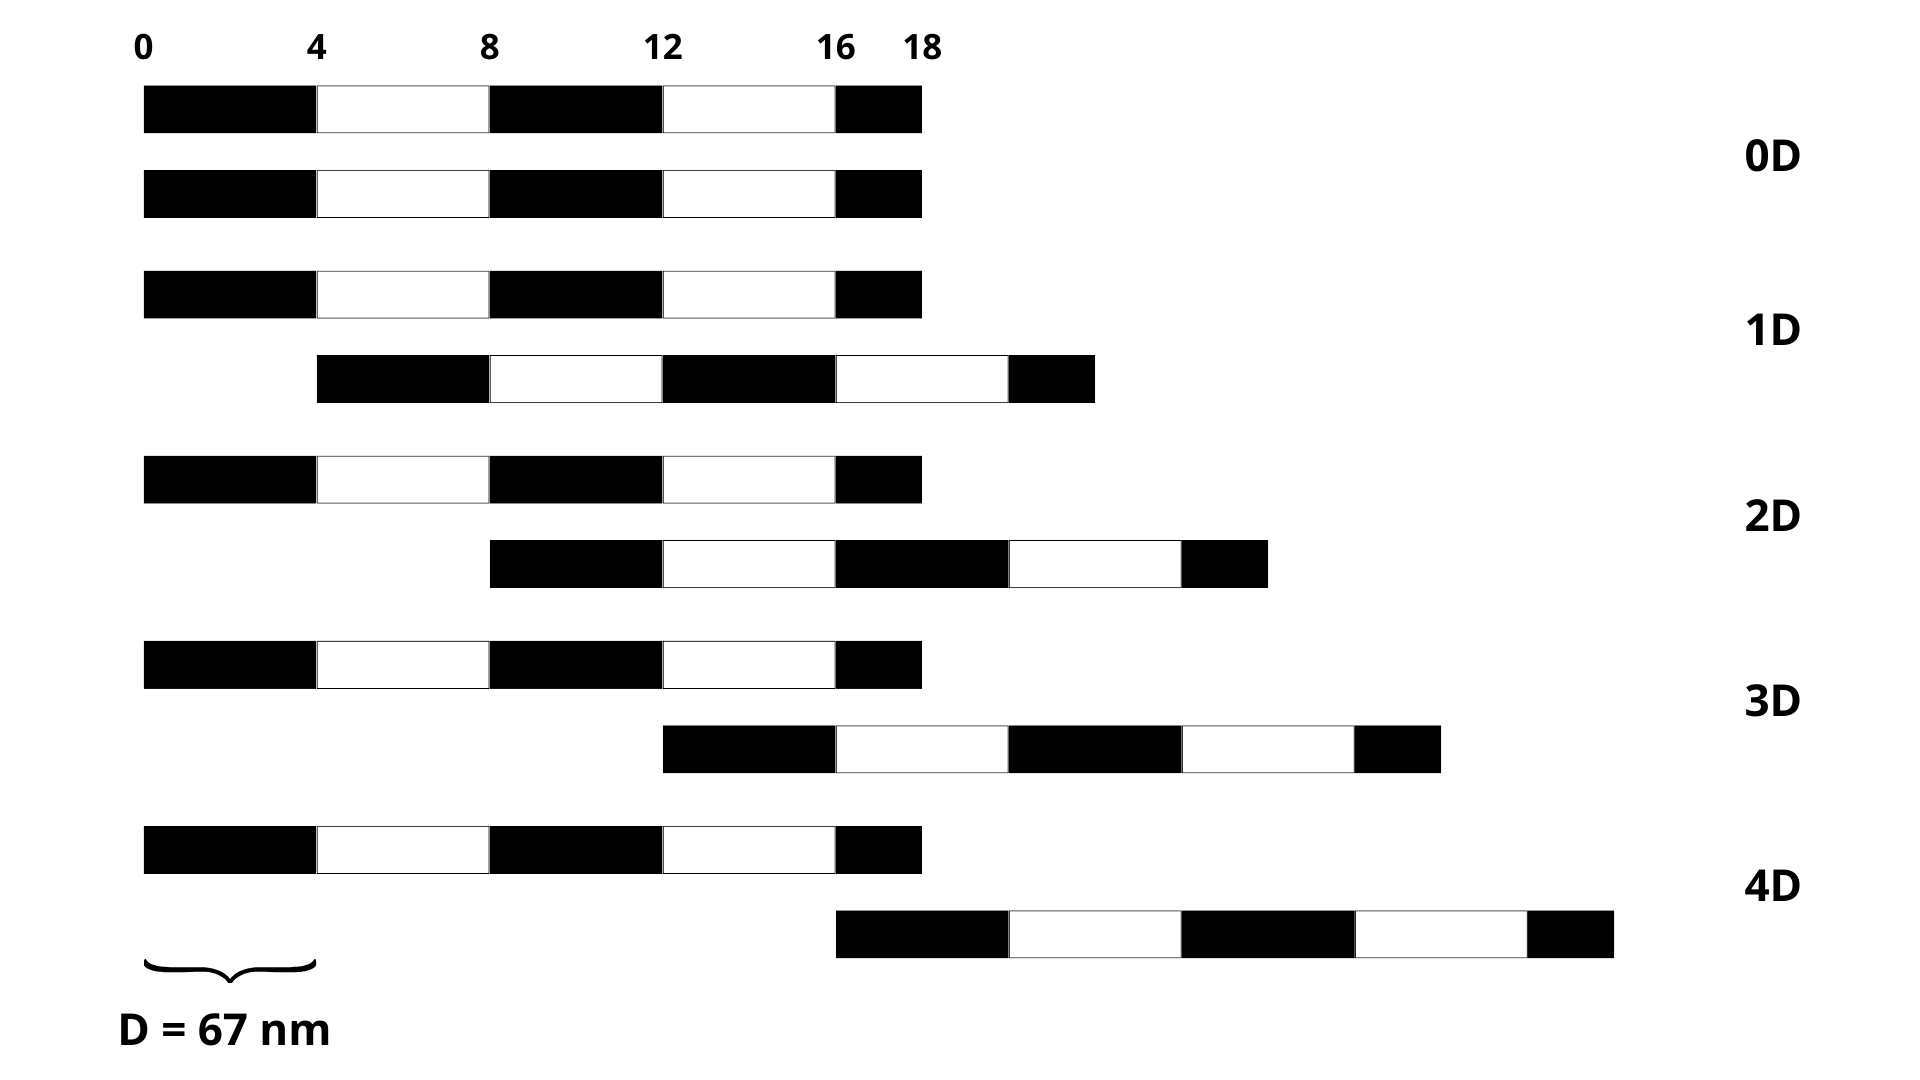
\includegraphics[width=\textwidth]{figures/specific_bind.png}
    
            \caption{.} 
    
            \label{M2}
        \end{figure}

        O processo de formação das fibrilas reais é dirigido por uma força hidrofóbica devido a interação entre as moléculas, de modo que elas 
        tentam minimizar sua superfície exposta para tal\cite{Kadler1987,Parkinson1995}. Para representar esse processo, utilizamos um algoritmo
        de difusão lateral sobre a superfície, que permite uma molécula recém agregada possa explorar a superfície, mantendo seu y fixo, para 
        encontrar um local que minimize sua superfície exposta\cite{GarcaRuiz1991}. Caso ocorra mais de um local, a primeira posição é mantida. 
        Esse movimento é controlado pelo parâmetro $T_{s}$ que define o número de tentativas que a molécula tem para explorar a superfície do 
        agregado\cite{Parkinson1995}.
     

        Com esse algorítimo, geramos $50$ fibrilas contendo $30.000$ bastões para diferentes valores de $T_{s}$ a fim de ver o efeito desse 
        parâmetro na morfologia das fibrilas. 


    \subsection{Propriedades das fibrilas}
        
        Para analisar as propriedades mecânicas das fibrilas, utilizamos um modelo mecânico probabilístico, visto que os agregados gerados 
        não possuem um carácter elástico para ser estudado usando modelos baseado em molas\cite{Parkinson1997,Saitoh2020MolecularDS}. 

        Primeiramente, iniciamos realizando o corte de um tronco de dimensão 17 x 201 x 17 em uma fibrila. Apos isso, nos fazemos uma limpeza 
        para garantir que nao ocorra a presença de moléculas desafixadas e determinar o esqueleto ativo. Para isso, nos consideramos que o 
        tronco é dividido em 201 camadas e que cada molécula possui parcelas, de tamanho unitario, em mais de uma camada. Iniciando pela primeira 
        camada, marcamos todas as moleculas como ativas, em seguida, verificamos se, em uma camada superior, uma particula pertencente a uma molecula 
        ativa possui uma particula vizinha inativa, se sim, ela é considerada ativada bem como todas as particulas, tanto acima quanto abaixo, pertencentes 
        aquela molécula. Repetimos esse procedimento até atingir a ultima camada. Esse procedimento pode ser visto na Figura \ref{M3}. Com essa 
        seleção de moléculas ativas, nos repetimos o procedimento, agora de cima para baixo, nesse conjunto até obtermos o esqueleto ativo, o conjunto 
        de moléculas pela qual uma força aplicada é capaz de percolar. 

        \begin{figure}[H]
            \centering
            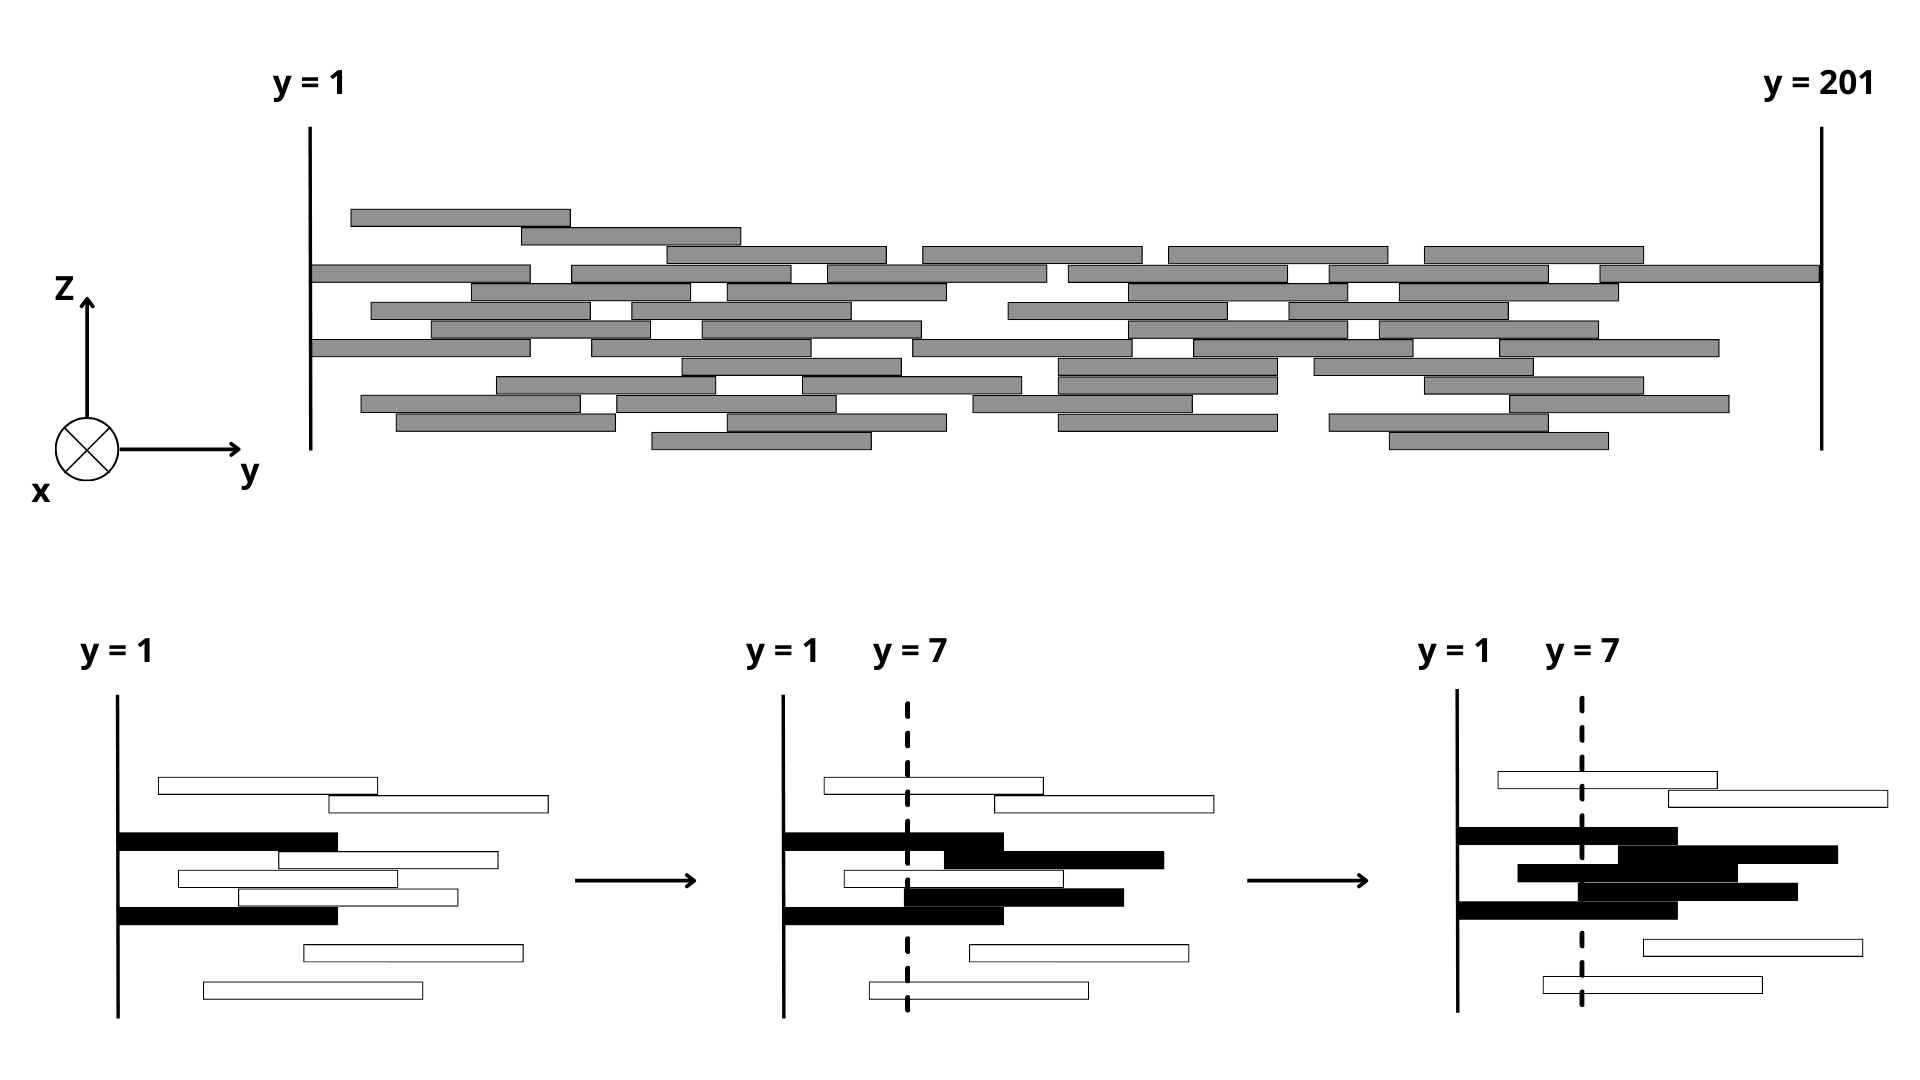
\includegraphics[width=\textwidth]{figures/esqueleto.png}
    
            \caption{.} 
    
            \label{M3}
        \end{figure}

        Uma vez que obtivemos o esqueleto ativo, nos atribuimos uma probabilidade $P_{R}$ a cada molécula. Uma vez que aplicamos uma força ao agregado,
        cada molécula sente uma fraça da mesma, onde ela é diminuida pelo número de particulas em uma dada camada. Dessa forma, todas as $M$ particulas 
        na i-ésima camada sentem uma força na forma 

        \begin{equation}
            \sigma_{i} = \frac{F}{M_{i}},
        \end{equation}
        \noindent com isso, a força que uma molécula sente no agregado é a media dos seus $\sigma_{i}$.

        As moléculas de colágeno possuem uma estrtura em tripla helice\cite{BRODSKY1997545}, dessa forma, a ruptura da propria molécula é mais imporvavel 
        de acontecer do que a quebra das ligações entre as moléculas\cite{Parkinson1997}. Portanto, nos consideramos uma probabilidade de ruptura para uma
        molécula ao inves de cada particula que a compõe. Nos tambem consideramos que o numero de ligações, responsaveis por manter a molécula presa no 
        esqueleto ativo, é igual somatorio do numero de particulas vizinhas em cada camada que a molécula está presente.

        Com isso, nossa probabilidade é determinada pela equação

        \begin{equation}
            P_{R} = (\frac{<\sigma>}{N\sigma_{s}})^{m},
        \end{equation}

        \noindent $N$ é o número de ligações que uma dada molécula possui, $\sigma_{s}$ é a força das ligações entre as moléculas e m é um fator de 
        amortecimento da energia\cite{Parkinson1997,2013}. Para todas as simulações, nos utilizamos $m$ = 2.

        A simulação consiste em aplicarmos umas força no esqueleto ativo, com isso, calculamos as probabilidades de cada molécula ser removida e sortíamos um número para ver se ocorre a ruptura. Caso ocorra pelo menos uma única quebra, repetimos o procedimento para uma dada força até que não mais ocorra rupturas. Nesse ponto, incrementamos a força em meio e repetimos a simulação. A fibrila se quebra se ocorrer a existência de pelo menos uma camada vazia.

        (fazer uma figura disso)

        Com isso, realizamos, para cada fibrila com um determinado valor de $T_{s}$, mil experimentos. Guardamos informações dos valores, para cada força, do número removido do esqueleto, bem quantas restaram.


\section{Resultados}
    \subsection{Morfologia das fibrilas}

    Os agregados gerados pelo modelo apresentam uma morfologia fibrilar, com características relevantes de sua forma 
    sendo determinadas pelo parâmetro \(T_{s}\). Podemos observar, na Figura \ref{R1}, a estrutura desses agregados 
    para os valores de \(T_{s} = 2\), baixa difusão, e \(T_{s} = 10000\), alta difusão lateral sobre a superfície. As 
    fibrilas com menor \(T_{s}\) apresentam uma forma mais aberta, enquanto para valores mais altos, observamos uma 
    forma mais compacta e regular. A coloração indica o quão antiga uma molécula é no agregado, indo do azul escuro, 
    mais antigas, para o amarelo, mais recentes. Nos agregados mais compactos, temos dificuldade em observar moléculas
    mais antigas visto que essas estão muito no interior da estrutura. Para as mais abertas, temos uma maior facilidade
    em observar moléculas mais antigas. Além disso, na visão lateral, observamos o comportamento alongado e com pontas 
    afinadas, típico de fibrilas reais. 

    \begin{figure}[H]
        \centering
        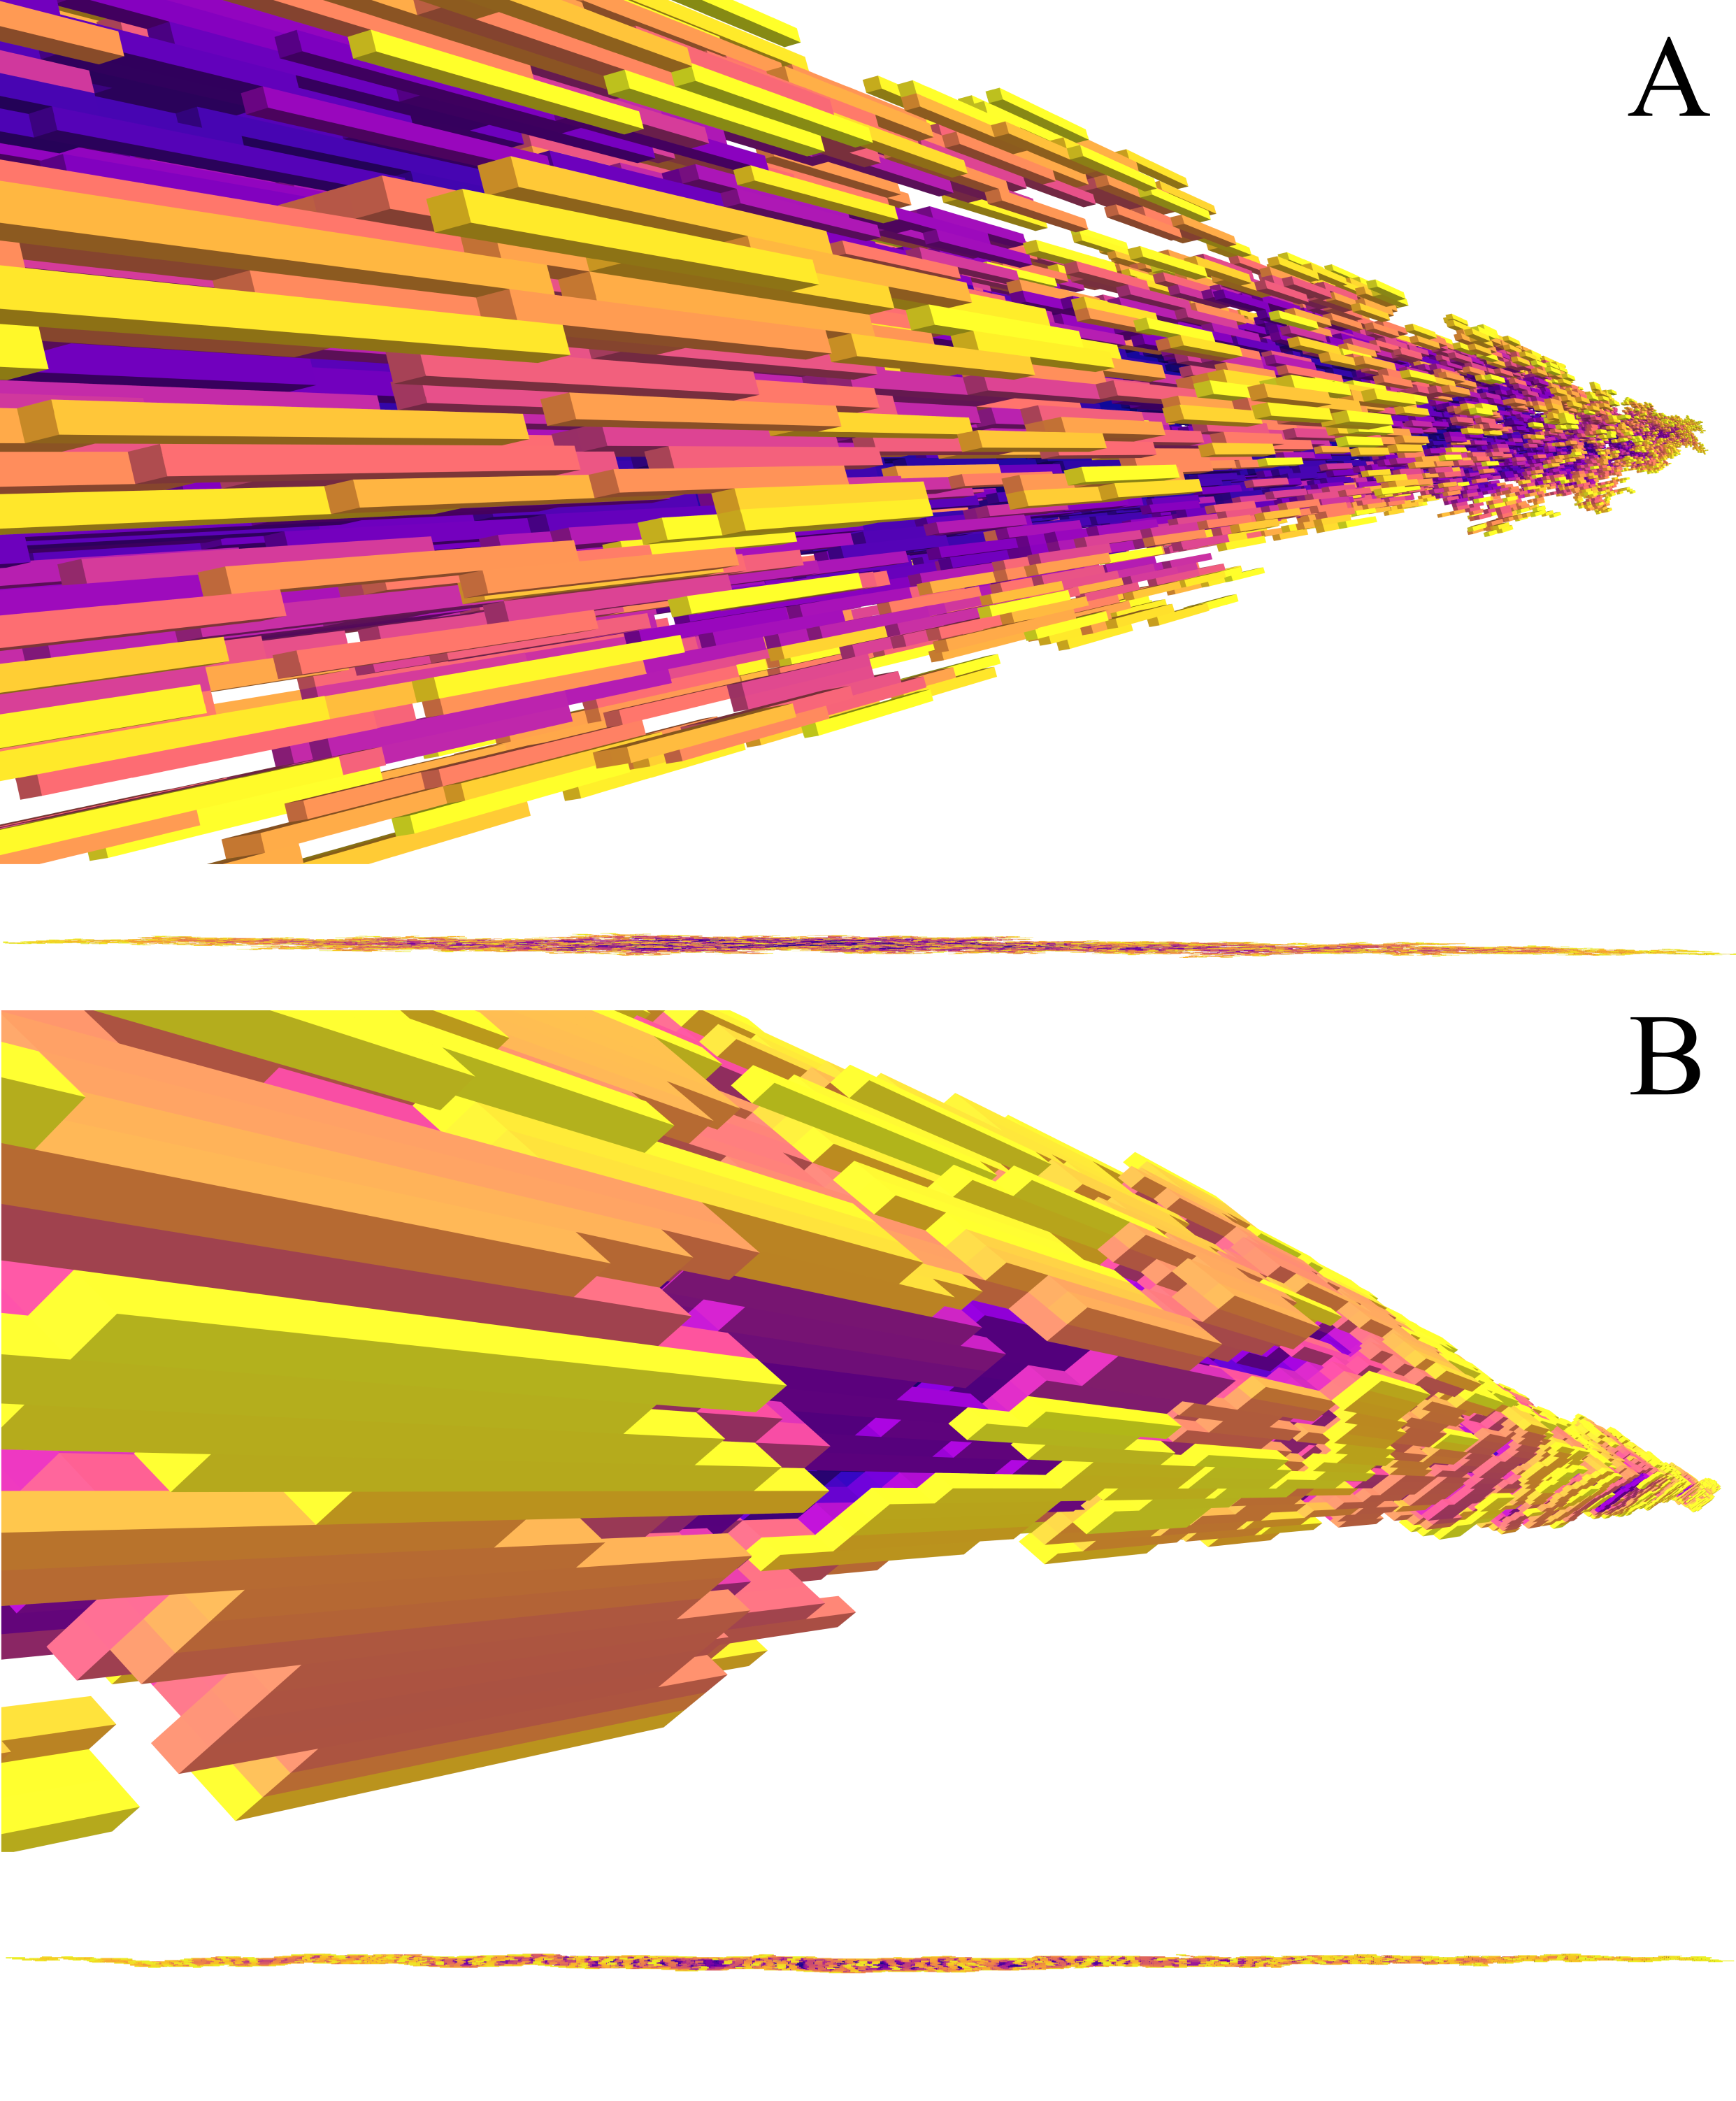
\includegraphics[width=\textwidth]{figures/fibrils.png}

        \caption{Visualização transversal e lateral das fibrilas geradas com o algoritmo de DLA contendo 30.000 moléculas.
        A coloração indica quão antigo é a molécula no agregado. Quanto mais pro azul escuro, 
        mais antigo no agregado, quanto mais para o amarelo, mais recente. 
        A) Fibrila gerada para \(T_{s}\) 2, baixa difusão. B) Fibrila gerada para \(T_{s}\) = 10000, alta difusão.} 

        \label{R1}
    \end{figure}

    O comprimento, o diâmetro e a densidade da região central das fibrilas são características influenciadas pelo 
    parâmetro \(T_{s}\). Na Tabela \ref{tab1}, podemos observar como essas dimensões se alteram, em média, com o 
    aumento desse parâmetro. O comprimento e a densidade tendem a aumentar com o incremento de \(T_{s}\), enquanto 
    o diâmetro tende a diminuir. Uma propriedade comum a essas medidas é que elas exibem um comportamento de 
    estabilização à medida que nos aproximamos de \(T_{s} = 512\); a partir desse ponto, elas oscilam em torno de um 
    valor médio. 

    \begin{table}[H]
        \caption{Valores médios dos comprimentos, diametros e densidade de fibrilas geradas para diferentes valores de \(T_{s}\).}

        \centering  % Mantém a tabela centralizada no texto
        \begin{tabular}{lccc}
        \hline
        \textbf{$T_{s}$} & \multicolumn{1}{c}{\textbf{Length(u.m)}} & \textbf{Ray(u.m)} & \textbf{Density(\% )} \\ \hline
        2                & 3668.36                                   & 32.40             & 0.17                  \\
        8                & 3695.16                                   & 28.68             & 0.25                  \\
        16               & 3764.27                                   & 24.63             & 0.34                  \\
        32               & 3808.68                                   & 21.67             & 0.46                  \\
        64               & 3891.56                                   & 17.6              & 0.57                  \\
        128              & 3928.6                                    & 16.06             & 0.62                  \\
        512              & 3913.24                                   & 14.07             & 0.66                  \\
        1024             & 3912.52                                   & 14.14             & 0.65                  \\
        4096             & 3892.28                                   & 14.06             & 0.66                  \\
        8192             & 3892.52                                   & 14.16             & 0.66                  \\
        10000            & 3917.16                                   & 13.94             & 0.65                  \\ \hline
        \multicolumn{1}{l}{Limit Upper} & 3905.54                    & 14.08             & 0.65                  \\ \hline
        \end{tabular}
        \label{tab1}  % Substitua 'meu_rótulo' pelo rótulo desejado para a referência cruzada
    \end{table}


    Outra característica desses agregados é a relação linear entre a massa e a distância até as pontas. Na Figura 
    \ref{R2}, observamos que, independentemente do valor de \(T_{s}\), todos os agregados exibem esse comportamento. 
    Tal característica é recorrentemente observada tanto em fibrilas reais quanto nas simuladas com este modelo 
    \cite{Parkinson1995,Kadler1987}. 


    \begin{figure}[H]
        \centering
        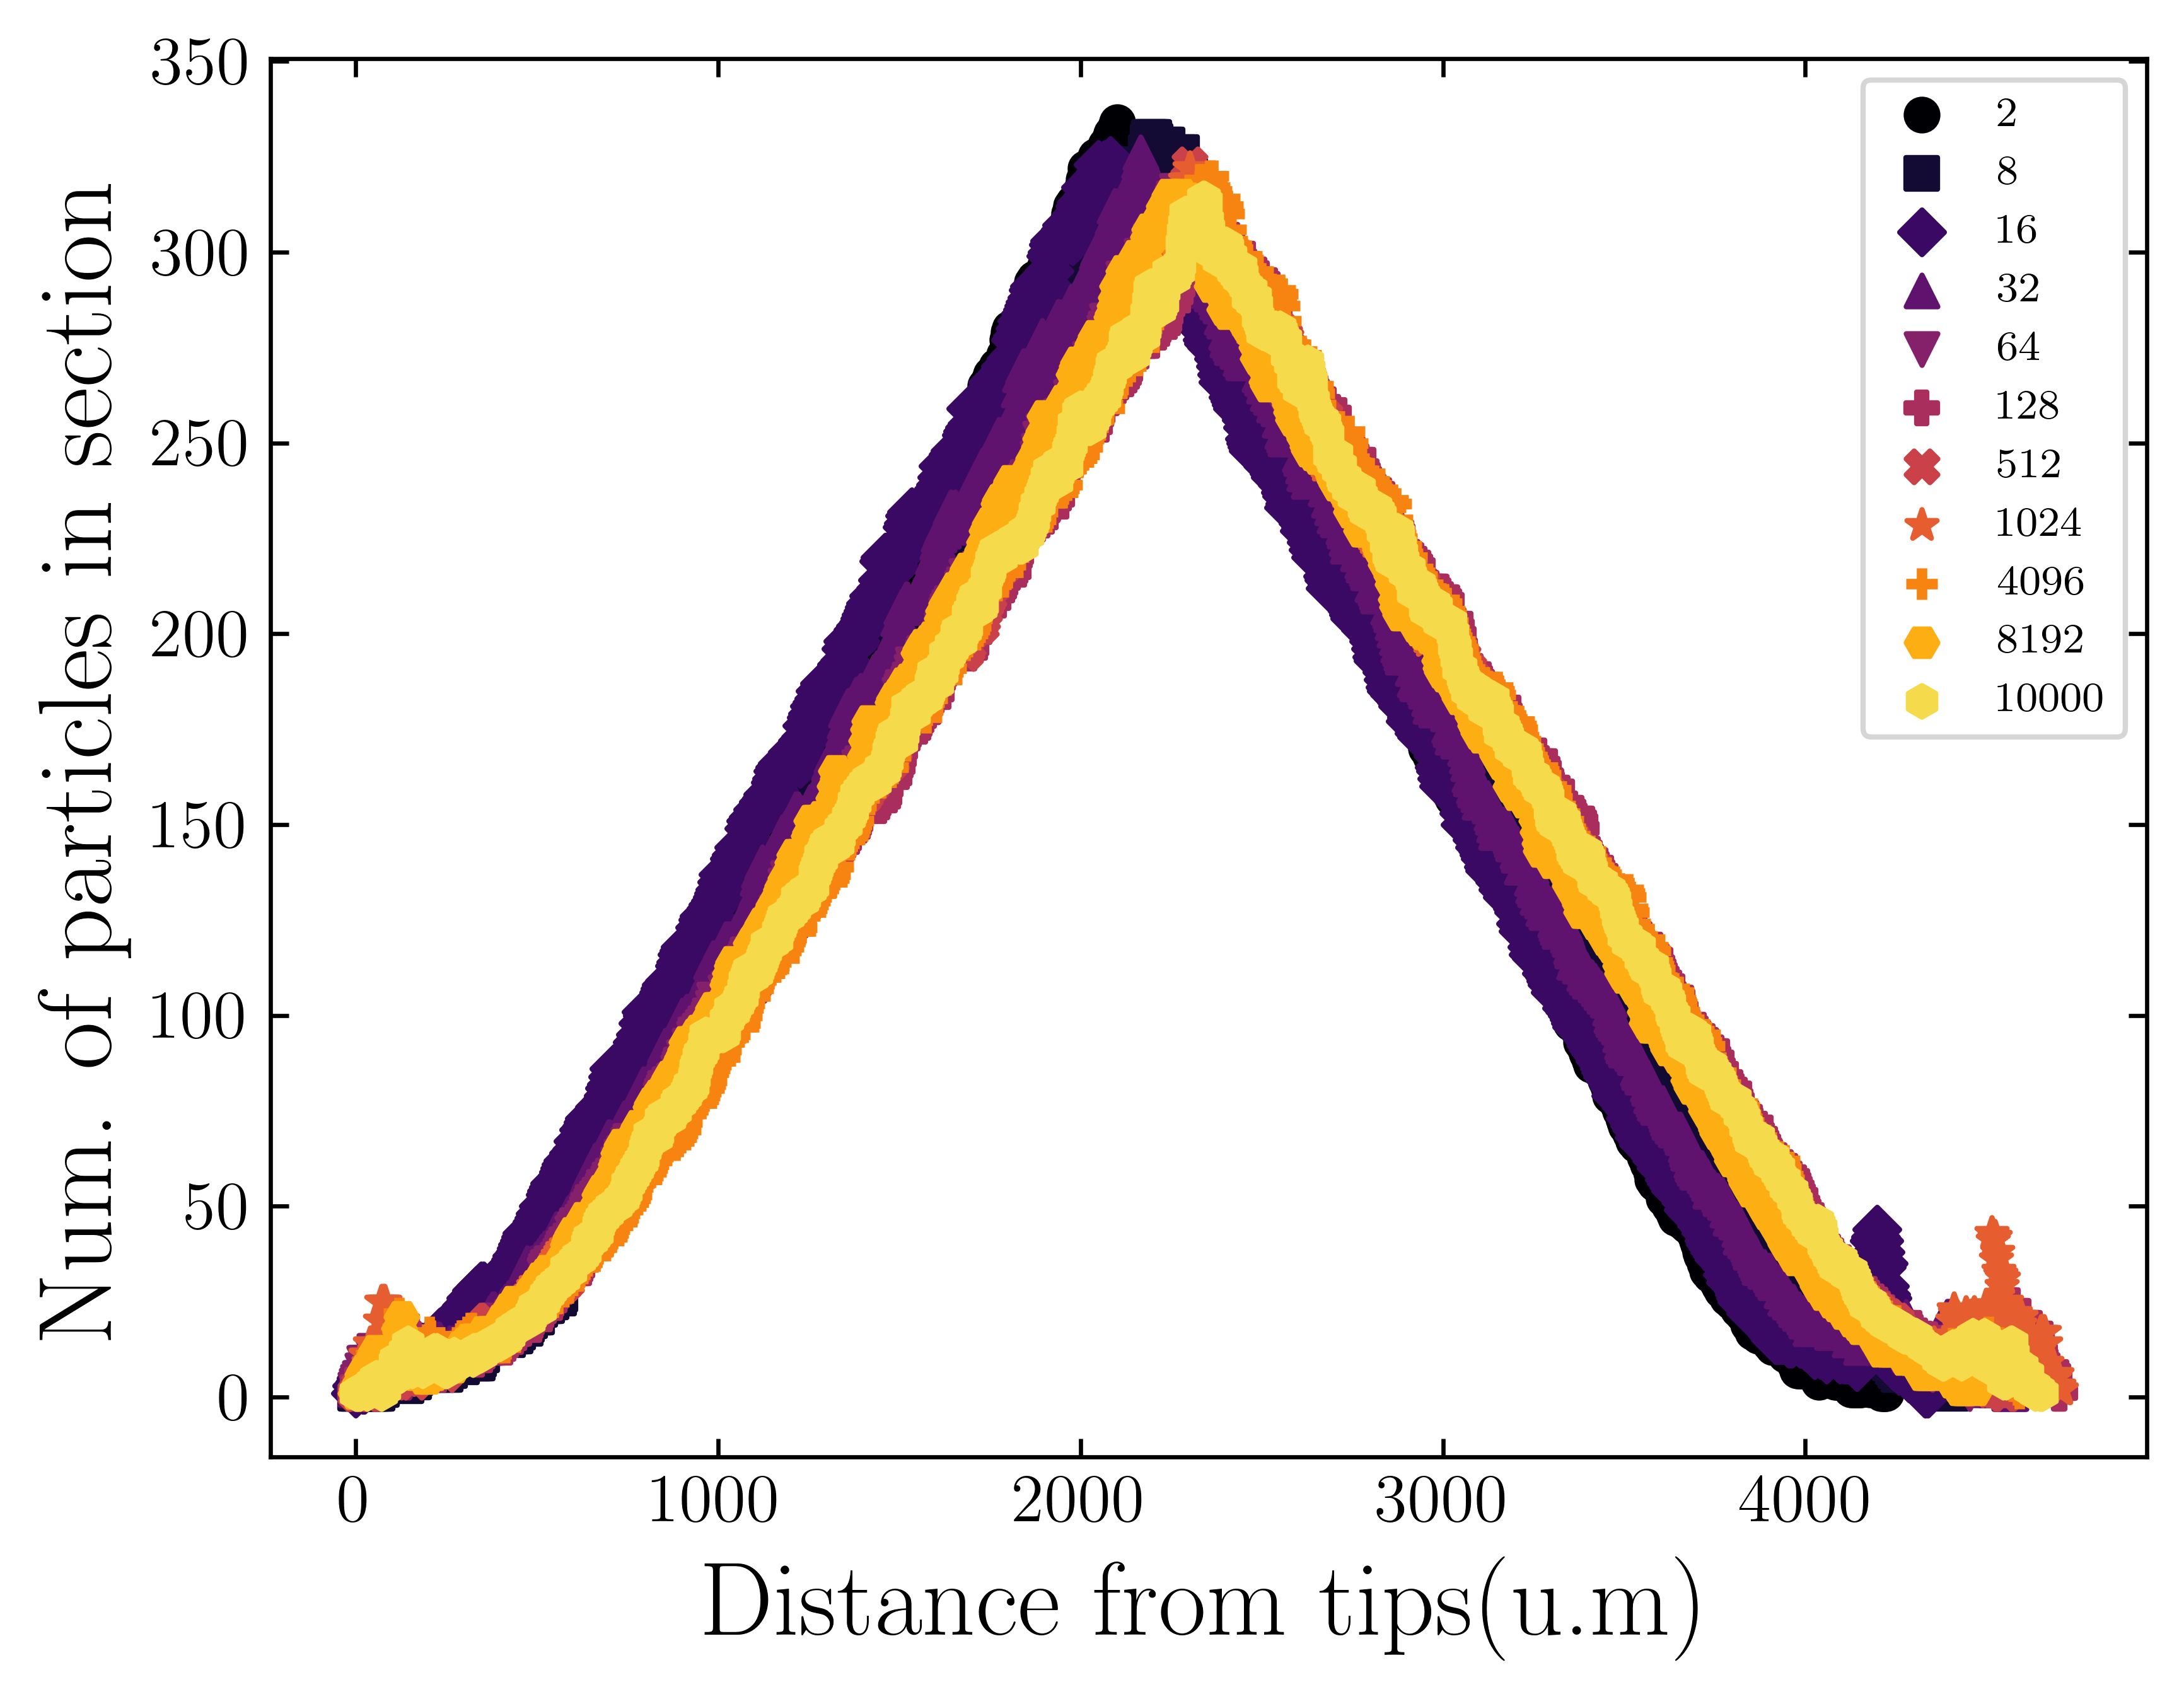
\includegraphics[width=\textwidth]{figures/tips.png}

        \caption{A quantidade de partículas por seção das fibrilas geradas segue uma relação linear da distancia em que 
        medimos para a ponta. Nos observamos que, partindo de uma ponta, a massa cresce linear até bem proximo da região
        central da fibrila. A medida que nos afastamos dessa região, a massa decaí linearmente. Esse comportamento foi 
        observado para todas as fibrilas, indicando que o parâmetro \(T_{s}\) não tem efeito sobre essa característica.} 

        \label{R2}
    \end{figure}


    Analisando a seção transversal das fibrilas, conforme ilustrado na Figura \ref{R3}, observamos que o aumento do 
    parâmetro \(T_{s}\) resulta na diminuição dos espaços vazios dentro da seção, levando à formação de agregados mais 
    compactos e quase completamente preenchidos. Devido a essa característica progressiva em função do parâmetro 
    \(T_{s}\), calculamos a dimensão fractal das seções e constatamos que, à medida que \(T_{s}\) aumenta, ocorre um 
    incremento no valor médio da dimensão fractal da seção até atingir uma saturação. Na Figura \ref{R4}, é evidente 
    que para valores mais baixos de \(T_{s}\), a dimensionalidade é próxima da observada em agregados gerados pelo 
    modelo de Agregação Limitada por Difusão (DLA) \cite{Witten1983}, que é de 1.71, remetendo ao nosso modelo de 
    formação. Enquanto isso, para valores mais elevados de \(T_{s}\), a dimensão fractal tende a estabilizar em valores 
    próximos a 1.93, que se assemelha muito à dimensão euclidiana para objetos bidimensionais. 

    \begin{figure}[H]
        \centering
        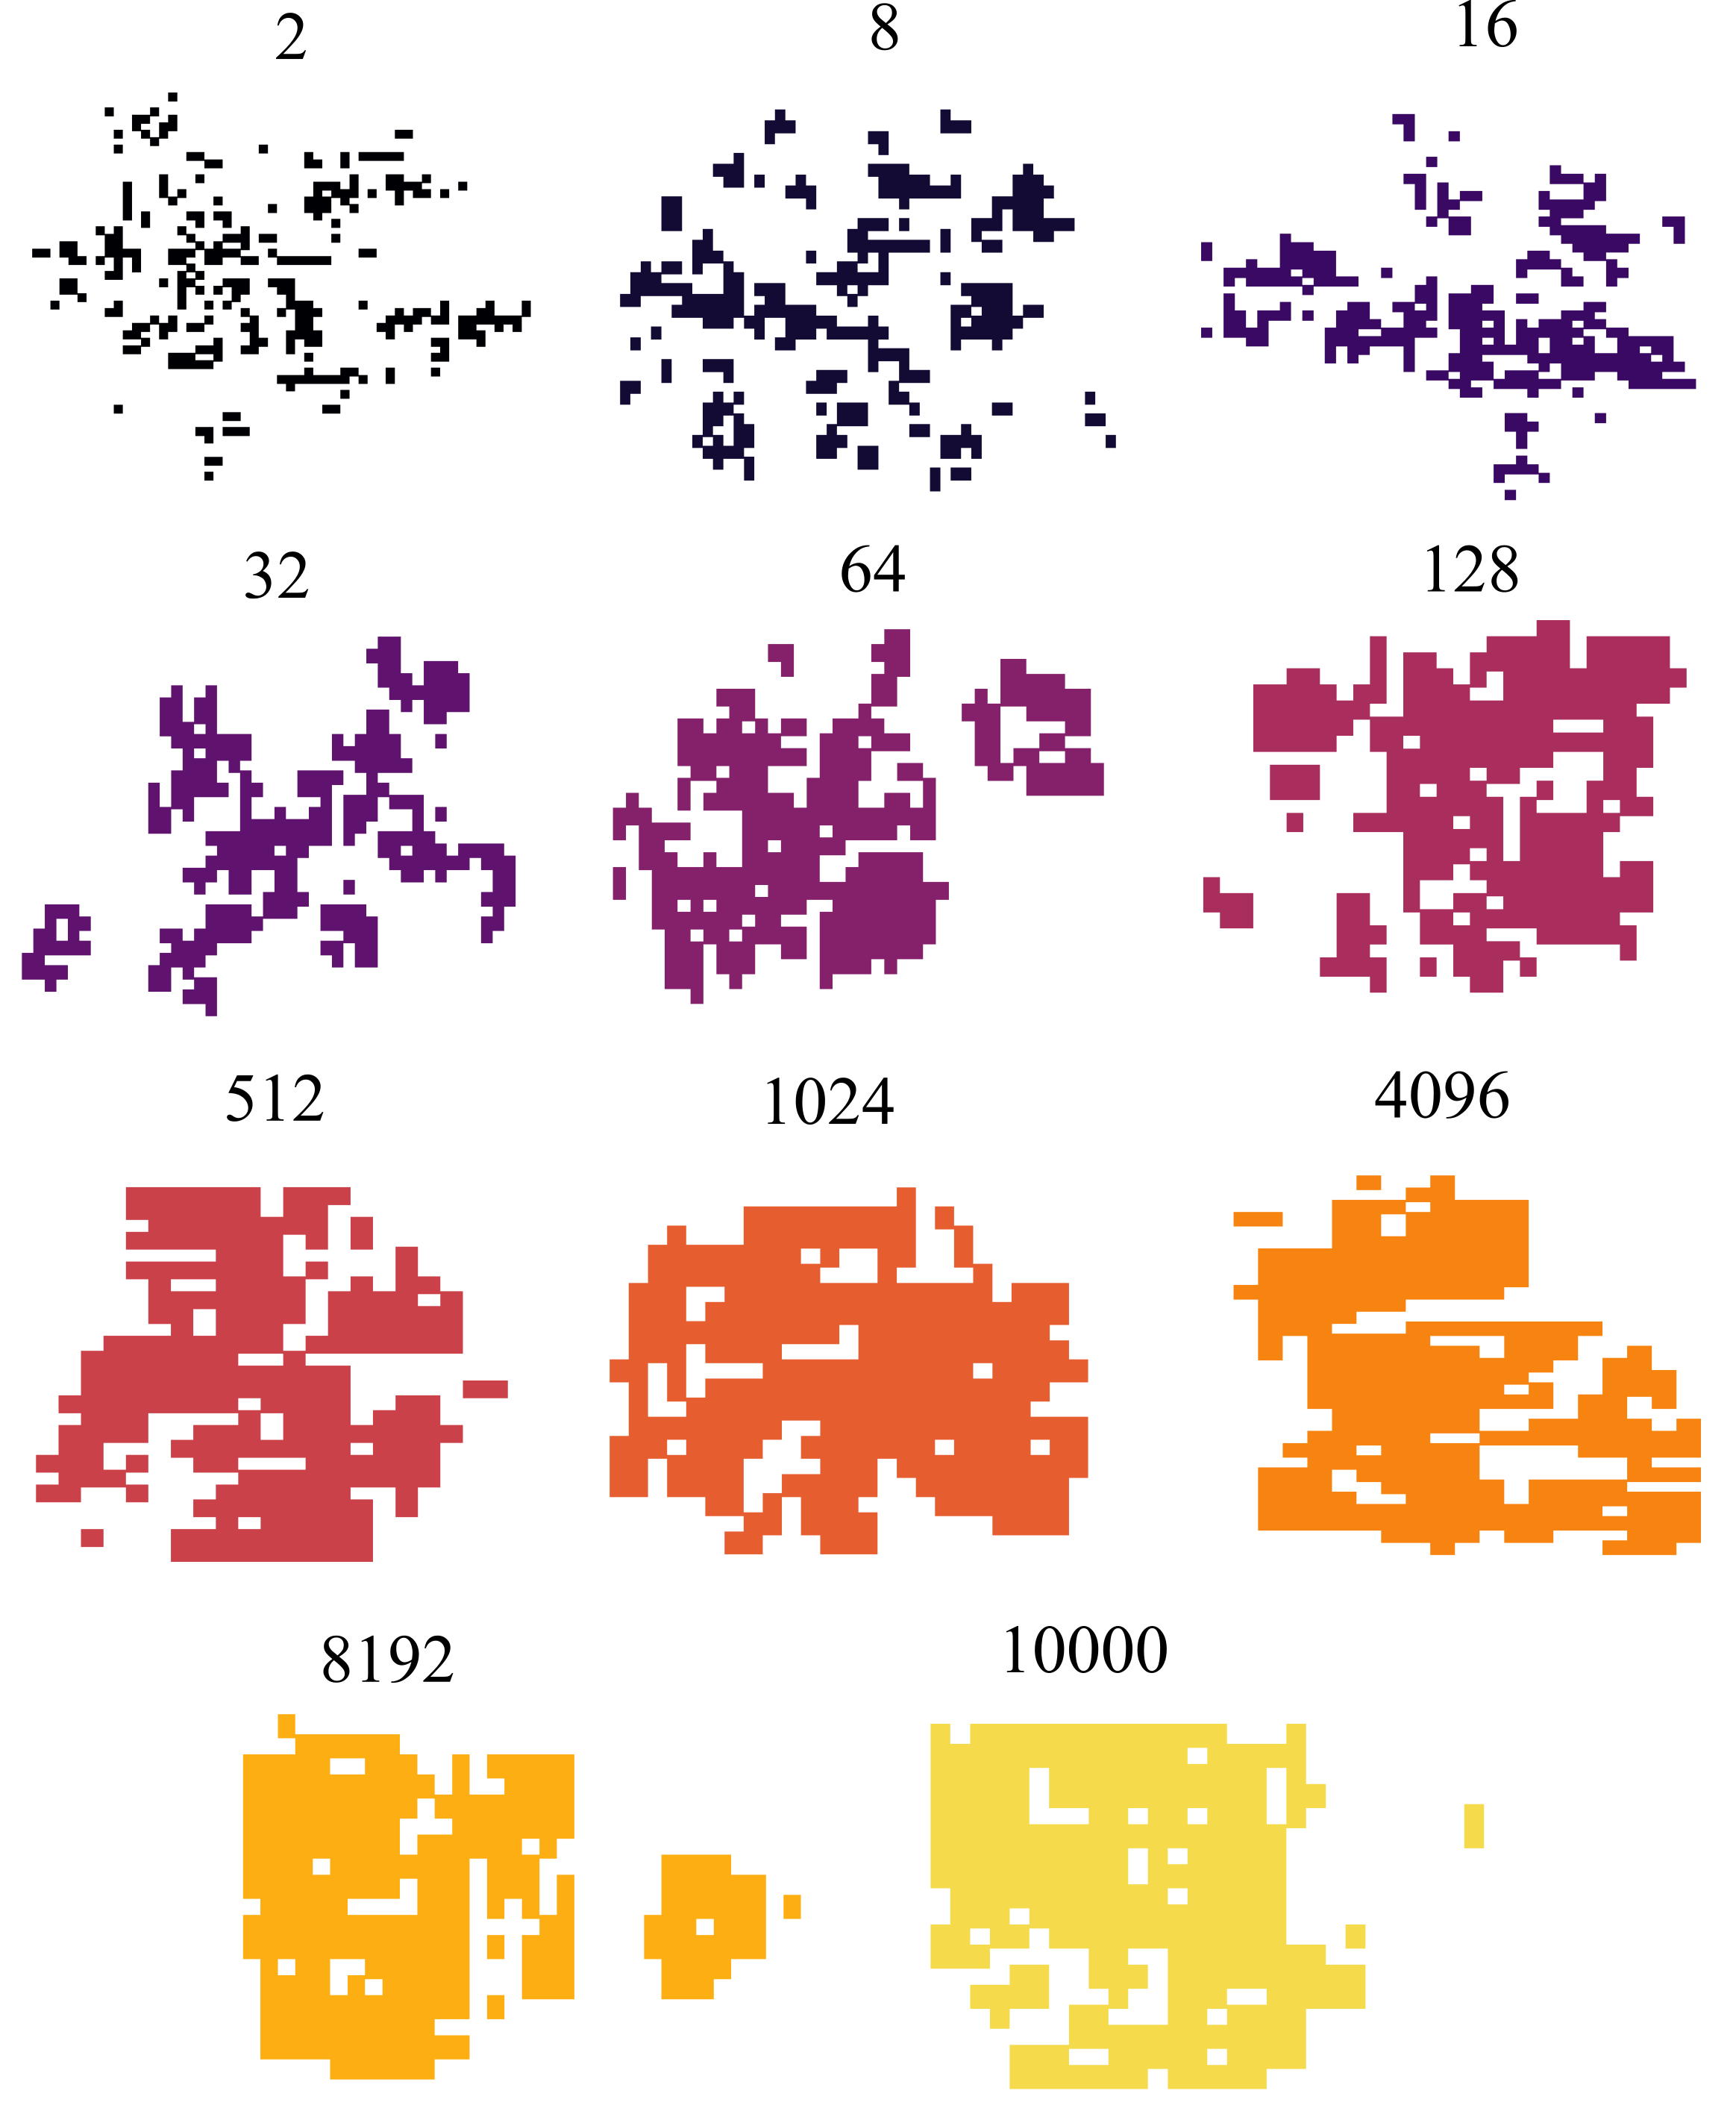
\includegraphics[width=\textwidth]{figures/cs_all.png}
        \caption{Variação da forma da seção transversal das fibrilas para diferentes valores de \(T_{s}\).} 
        \label{R3}
    \end{figure}

    \begin{figure}[H]
        \centering
        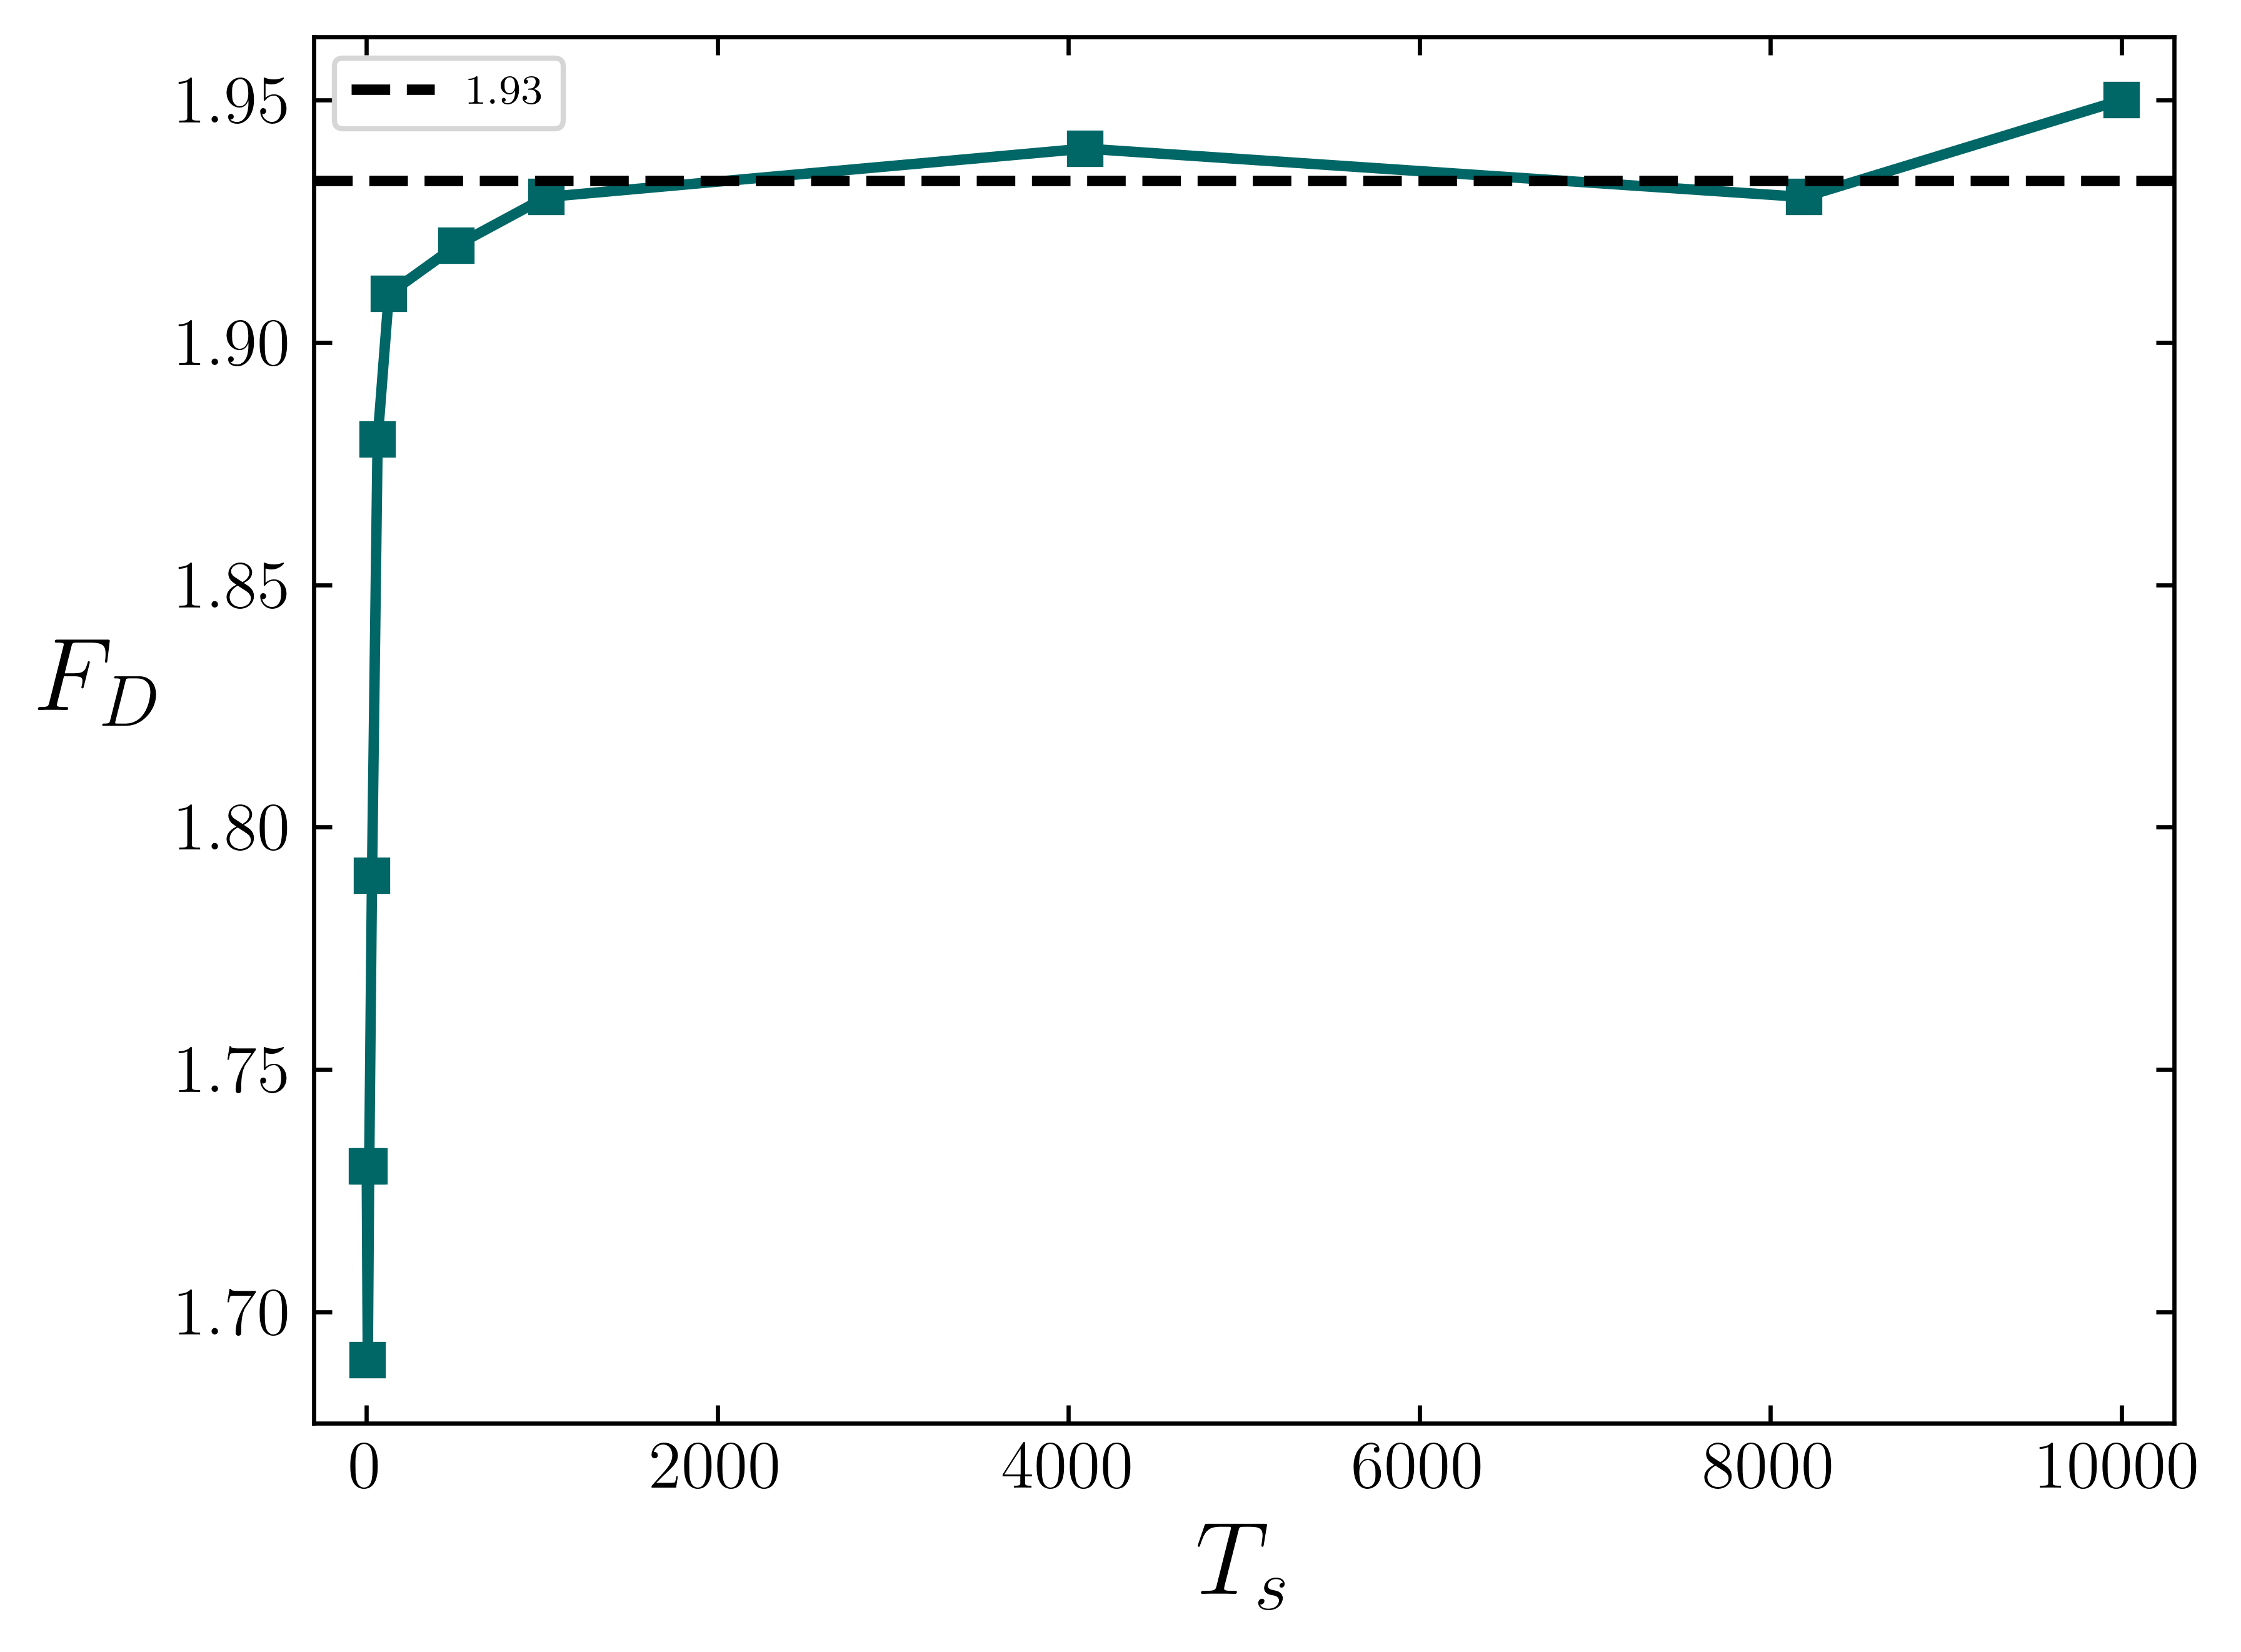
\includegraphics[width=\textwidth]{figures/dim_frac.png}

        \caption{ Dimensão fractal média da sesção transversal em função do parâmetro \(T_{s}\).} 

        \label{R4}
    \end{figure}


    \subsection{Propriedades mecânicas}

    Para compreender como nosso agregado responde à aplicação de uma força axial, avaliamos como o número de 
    moléculas na fibrila varia com a força. Na Figura \ref{R5}, apresentamos a curva de stress-strain para agregados 
    gerados com diferentes valores de \(T_{s}\). Observamos que o aumento desse parâmetro influencia no incremento da 
    tensão máxima de ruptura. No entanto, a partir de \(T_{s} = 512\), esses valores se tornam bastante próximos e as 
    curvas começam a se sobrepor. Comumente, esperaríamos que essas curvas crescessem de forma mais abrupta até o valor
    máximo, o que não é observado aqui. Esse comportamento mais suave até o valor limite é uma consequência do módulo 
    de Weibull que utilizamos no modelo. Para valores baixos, a curva resultante é não determinística 
    \cite{Parkinson1997}. A tensão máxima suportada que encontramos foi de 45,6 MPa, valor muito próximo ao encontrado 
    por Yang et al. \cite{YANG2012148} ao analisar fibrilas reconstituídas do tendão de Aquiles bovino purificado. 
    Em contraste, no trabalho de Yamamoto \cite{Noritaka}, foram utilizadas fibrilas isoladas do fascículo dos tendões 
    da cauda de ratos, obtendo um valor de 100 \(\pm\) 32 MPa. A discrepância em relação ao nosso valor pode estar 
    associada à dimensão das fibrilas utilizadas por ele, que apresentavam um diâmetro significativamente maior do que 
    as modeladas neste trabalho.

    \begin{figure}[H]
        \centering
        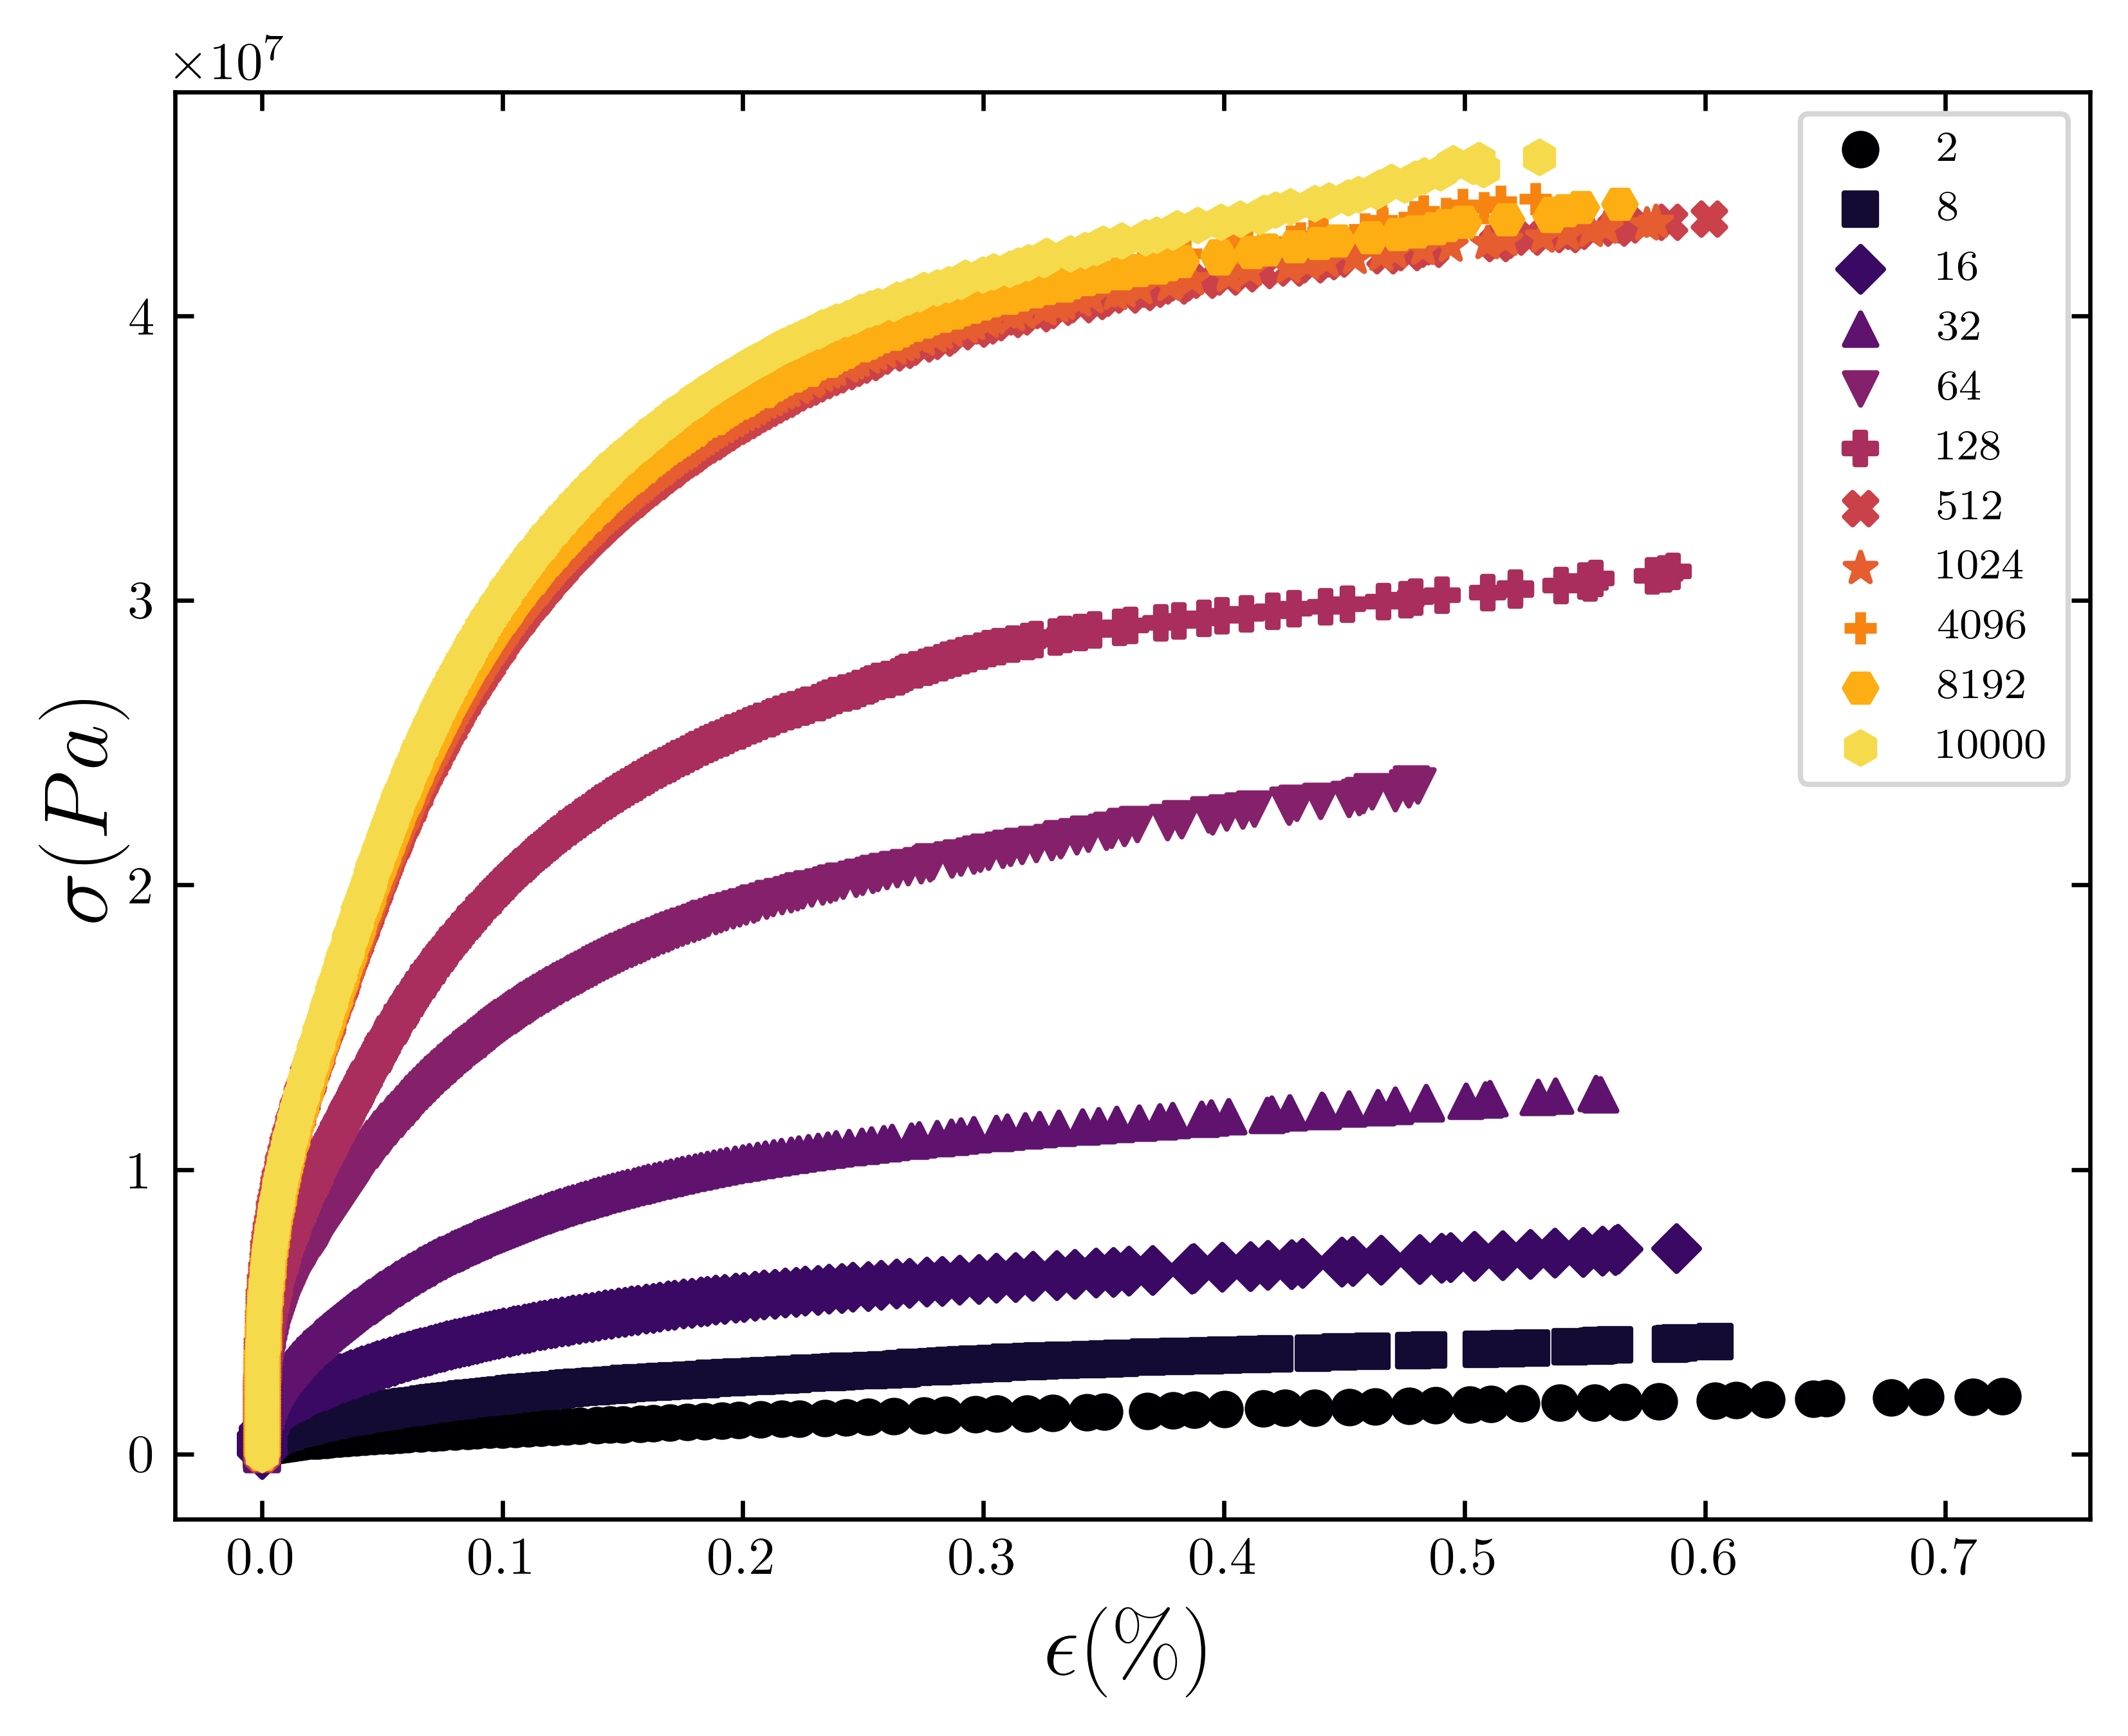
\includegraphics[width=\textwidth]{figures/stress_strain.png}

        \caption{Tensão em função da deformação da fibrila para diferentes valores de \(T_{s}\).} 

        \label{R5}
    \end{figure}

    Na Figura \ref{R6}, podemos observar como os valores de tensão máxima suportada variam com um parâmetro 
    importante das fibrilas, a densidade. Escolhemos essa análise visto que o comportamento de \(\sigma\) e da 
    densidade, \(\rho\), exibem formas semelhantes quando analisados em função de \(T_{s}\). Identificamos um 
    comportamento exponencial no aumento da tensão máxima até um limite superior de 44,1 MPa. A saturação da 
    densidade ocorre em 65\%, valor este próximo ao encontrado por Parkinson et al.\cite{Parkinson1995} com esse 
    modelo, porém um pouco abaixo do determinado por Katz et al.\cite{KATZ1973351}, que calculou experimentalmente 
    cerca de 80\% do espaço disponível ocupado para as fibrilas de colágeno. Com base nessa característica de 
    saturação, consideramos que, dado o custo computacional elevado, este modelo pode ser executado, para os parâmetros 
    que inicialmente utilizamos, com \(T_{s}=512\), uma vez que nesse ponto já obtemos fibrilas com os valores de 
    interesse médios equivalentes para valores superiores desse parâmetro. 



    \begin{figure}[H]
        \centering
        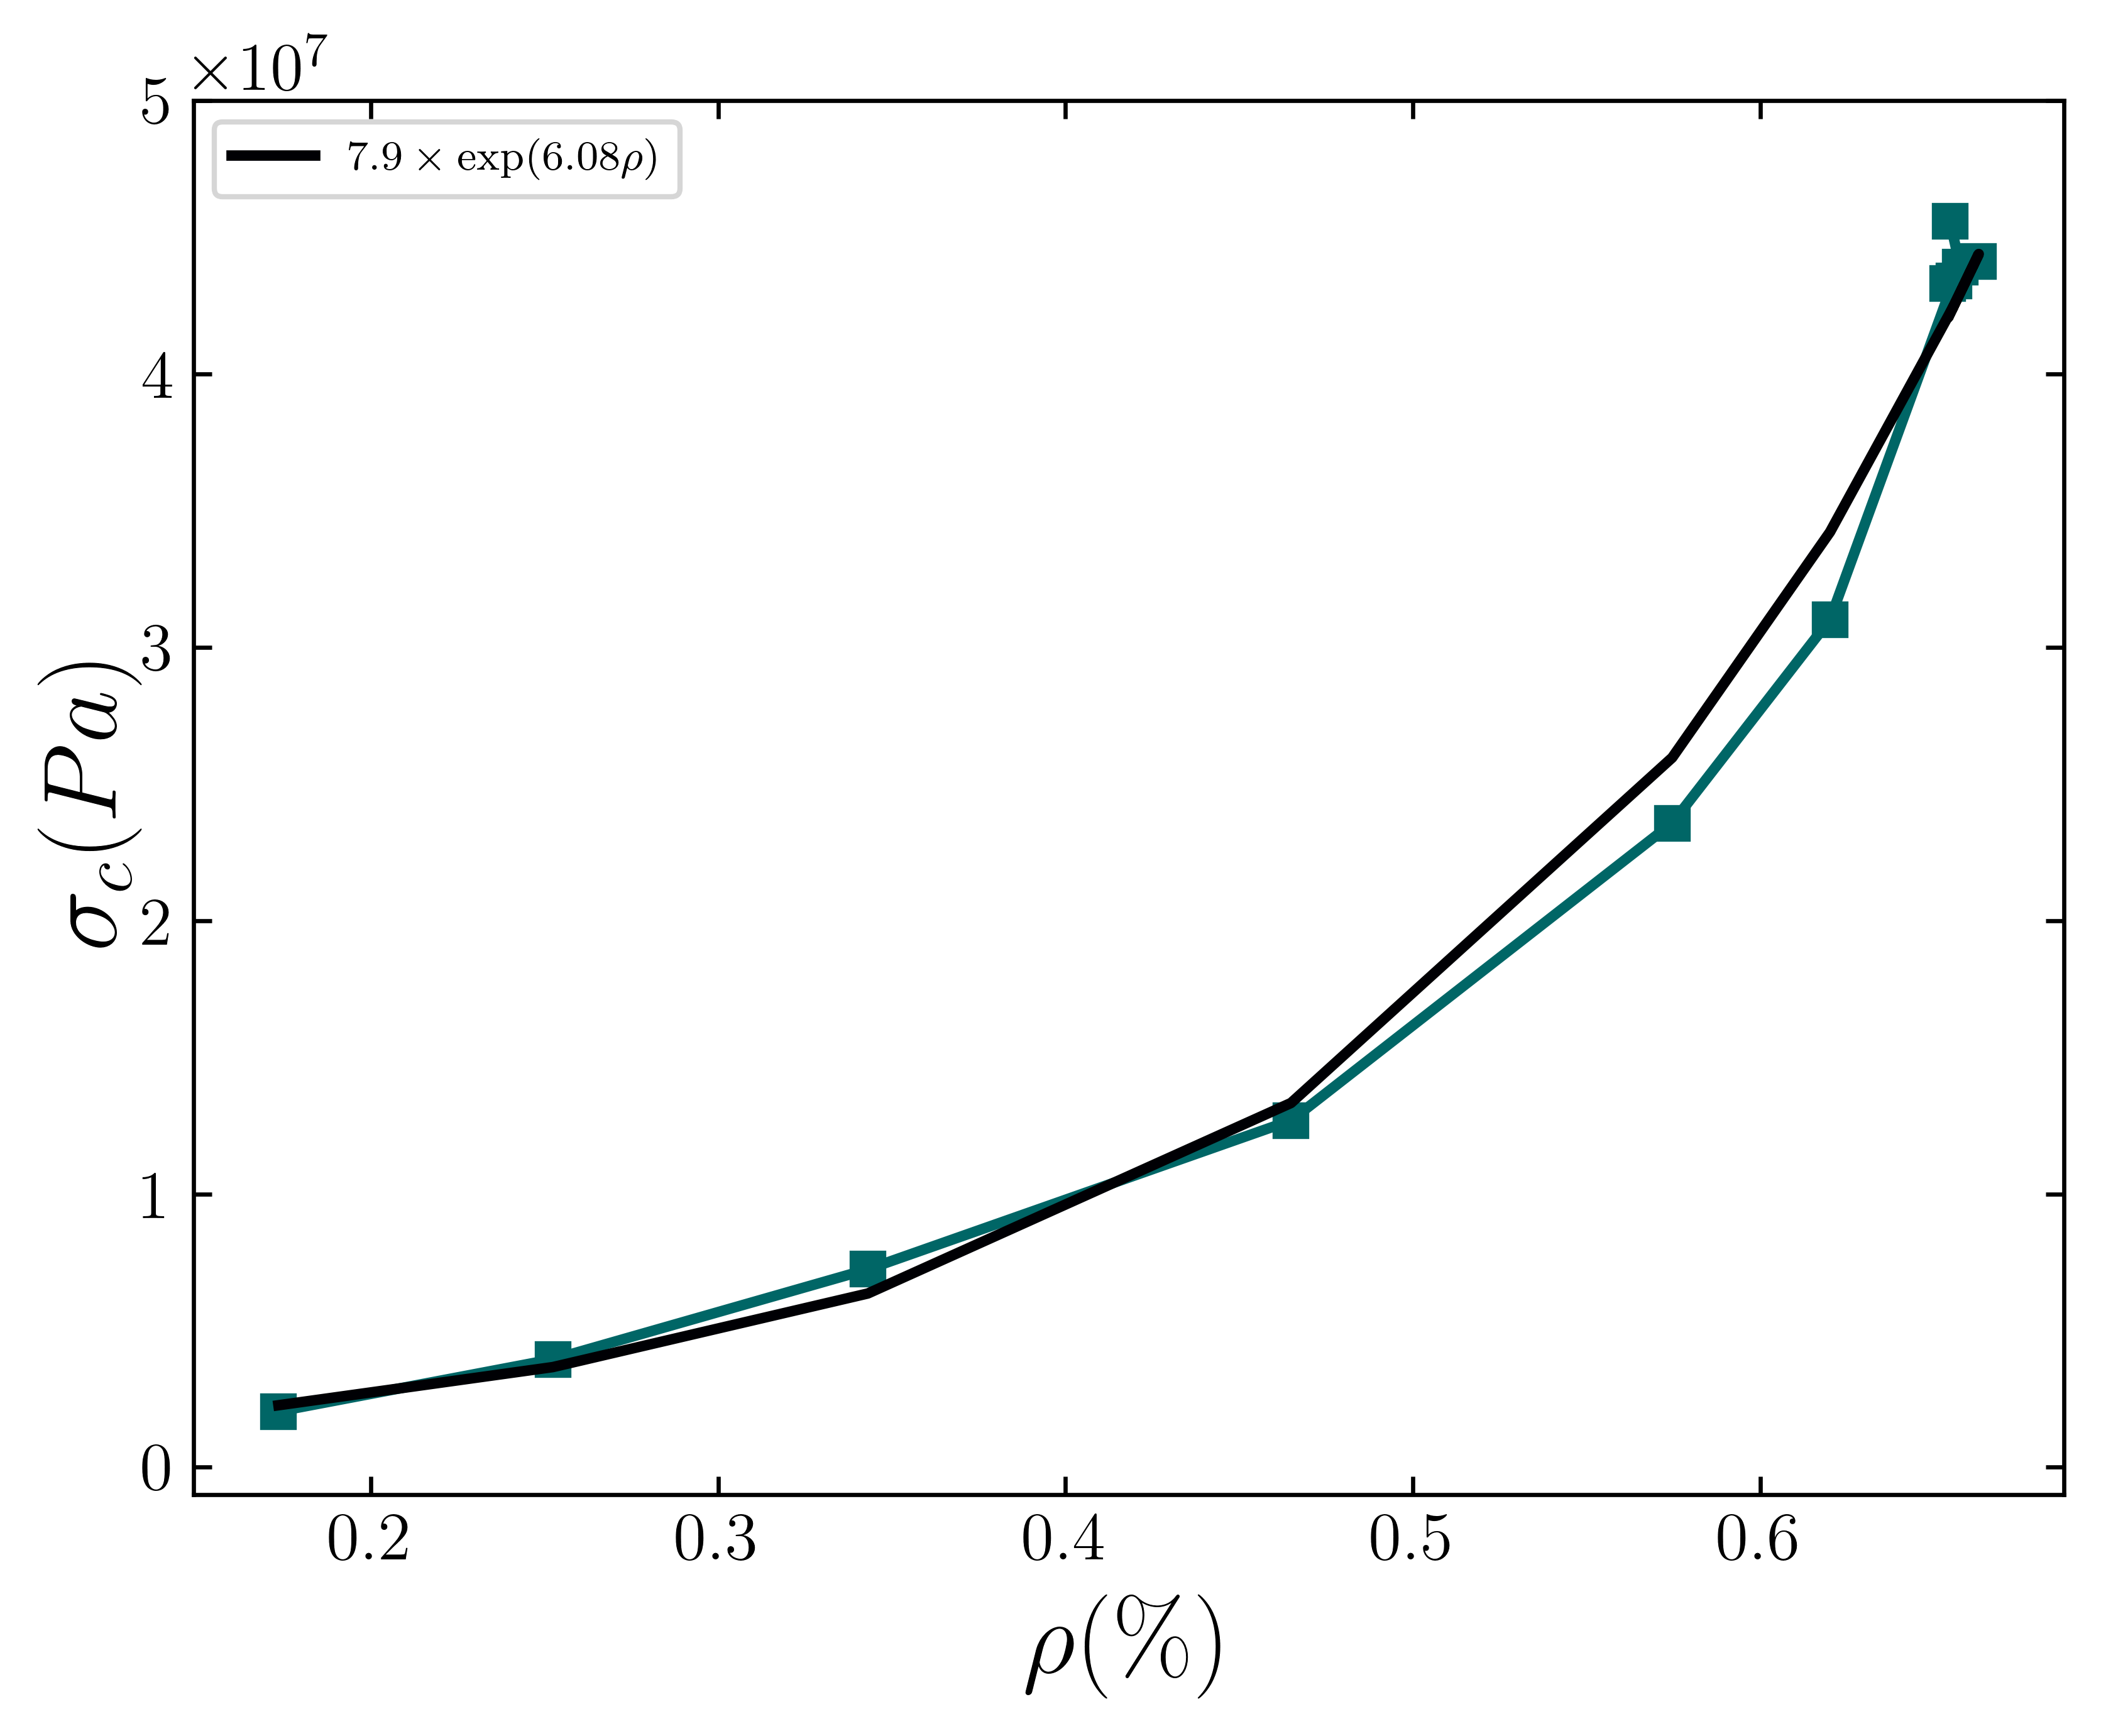
\includegraphics[width=\textwidth]{figures/sigma_rho.png}

        \caption{Tensão crítica em função da densidade. Observamos que esse valor cresce exponencialmente com a 
        densidade até ambos os parâmetros atingirem um limite superior.} 


        \label{R6}
    \end{figure}

    Ao analisar como o processo de ruptura ocorre no nosso modelo, bem como em outros, constatamos que a 
    redistribuição de tensão, para uma mesma força, pode levar à ocorrência de rupturas em cascata. Na Figura 
    \ref{R7}, apresentamos a distribuição das avalanches de ruptura em função do seu tamanho. É possível observar a 
    existência de duas ordens de grandeza bem definidas; após isso, os dados são afetados pelo efeito de tamanho 
    finito. Analisando a região de interesse, até próximo de \(10^{2.5}\), conseguimos determinar o expoente das leis 
    de escala de modo que eles aumentam com o crescimento de \(T_{s}\). Este comportamento é compreensível ao 
    considerarmos que a densidade aumenta com este parâmetro, resultando em mais moléculas para contribuir com os 
    tamanhos das avalanches. Assim, temos que as avalanches durante o processo de ruptura são independentes do tamanho 
    do sistema; contudo, elas são influenciadas pelo quão compacta é a fibrila, com o expoente \(\gamma\) variando de 
    -1.94 até -2.60. 


    \begin{figure}[H]
        \centering
        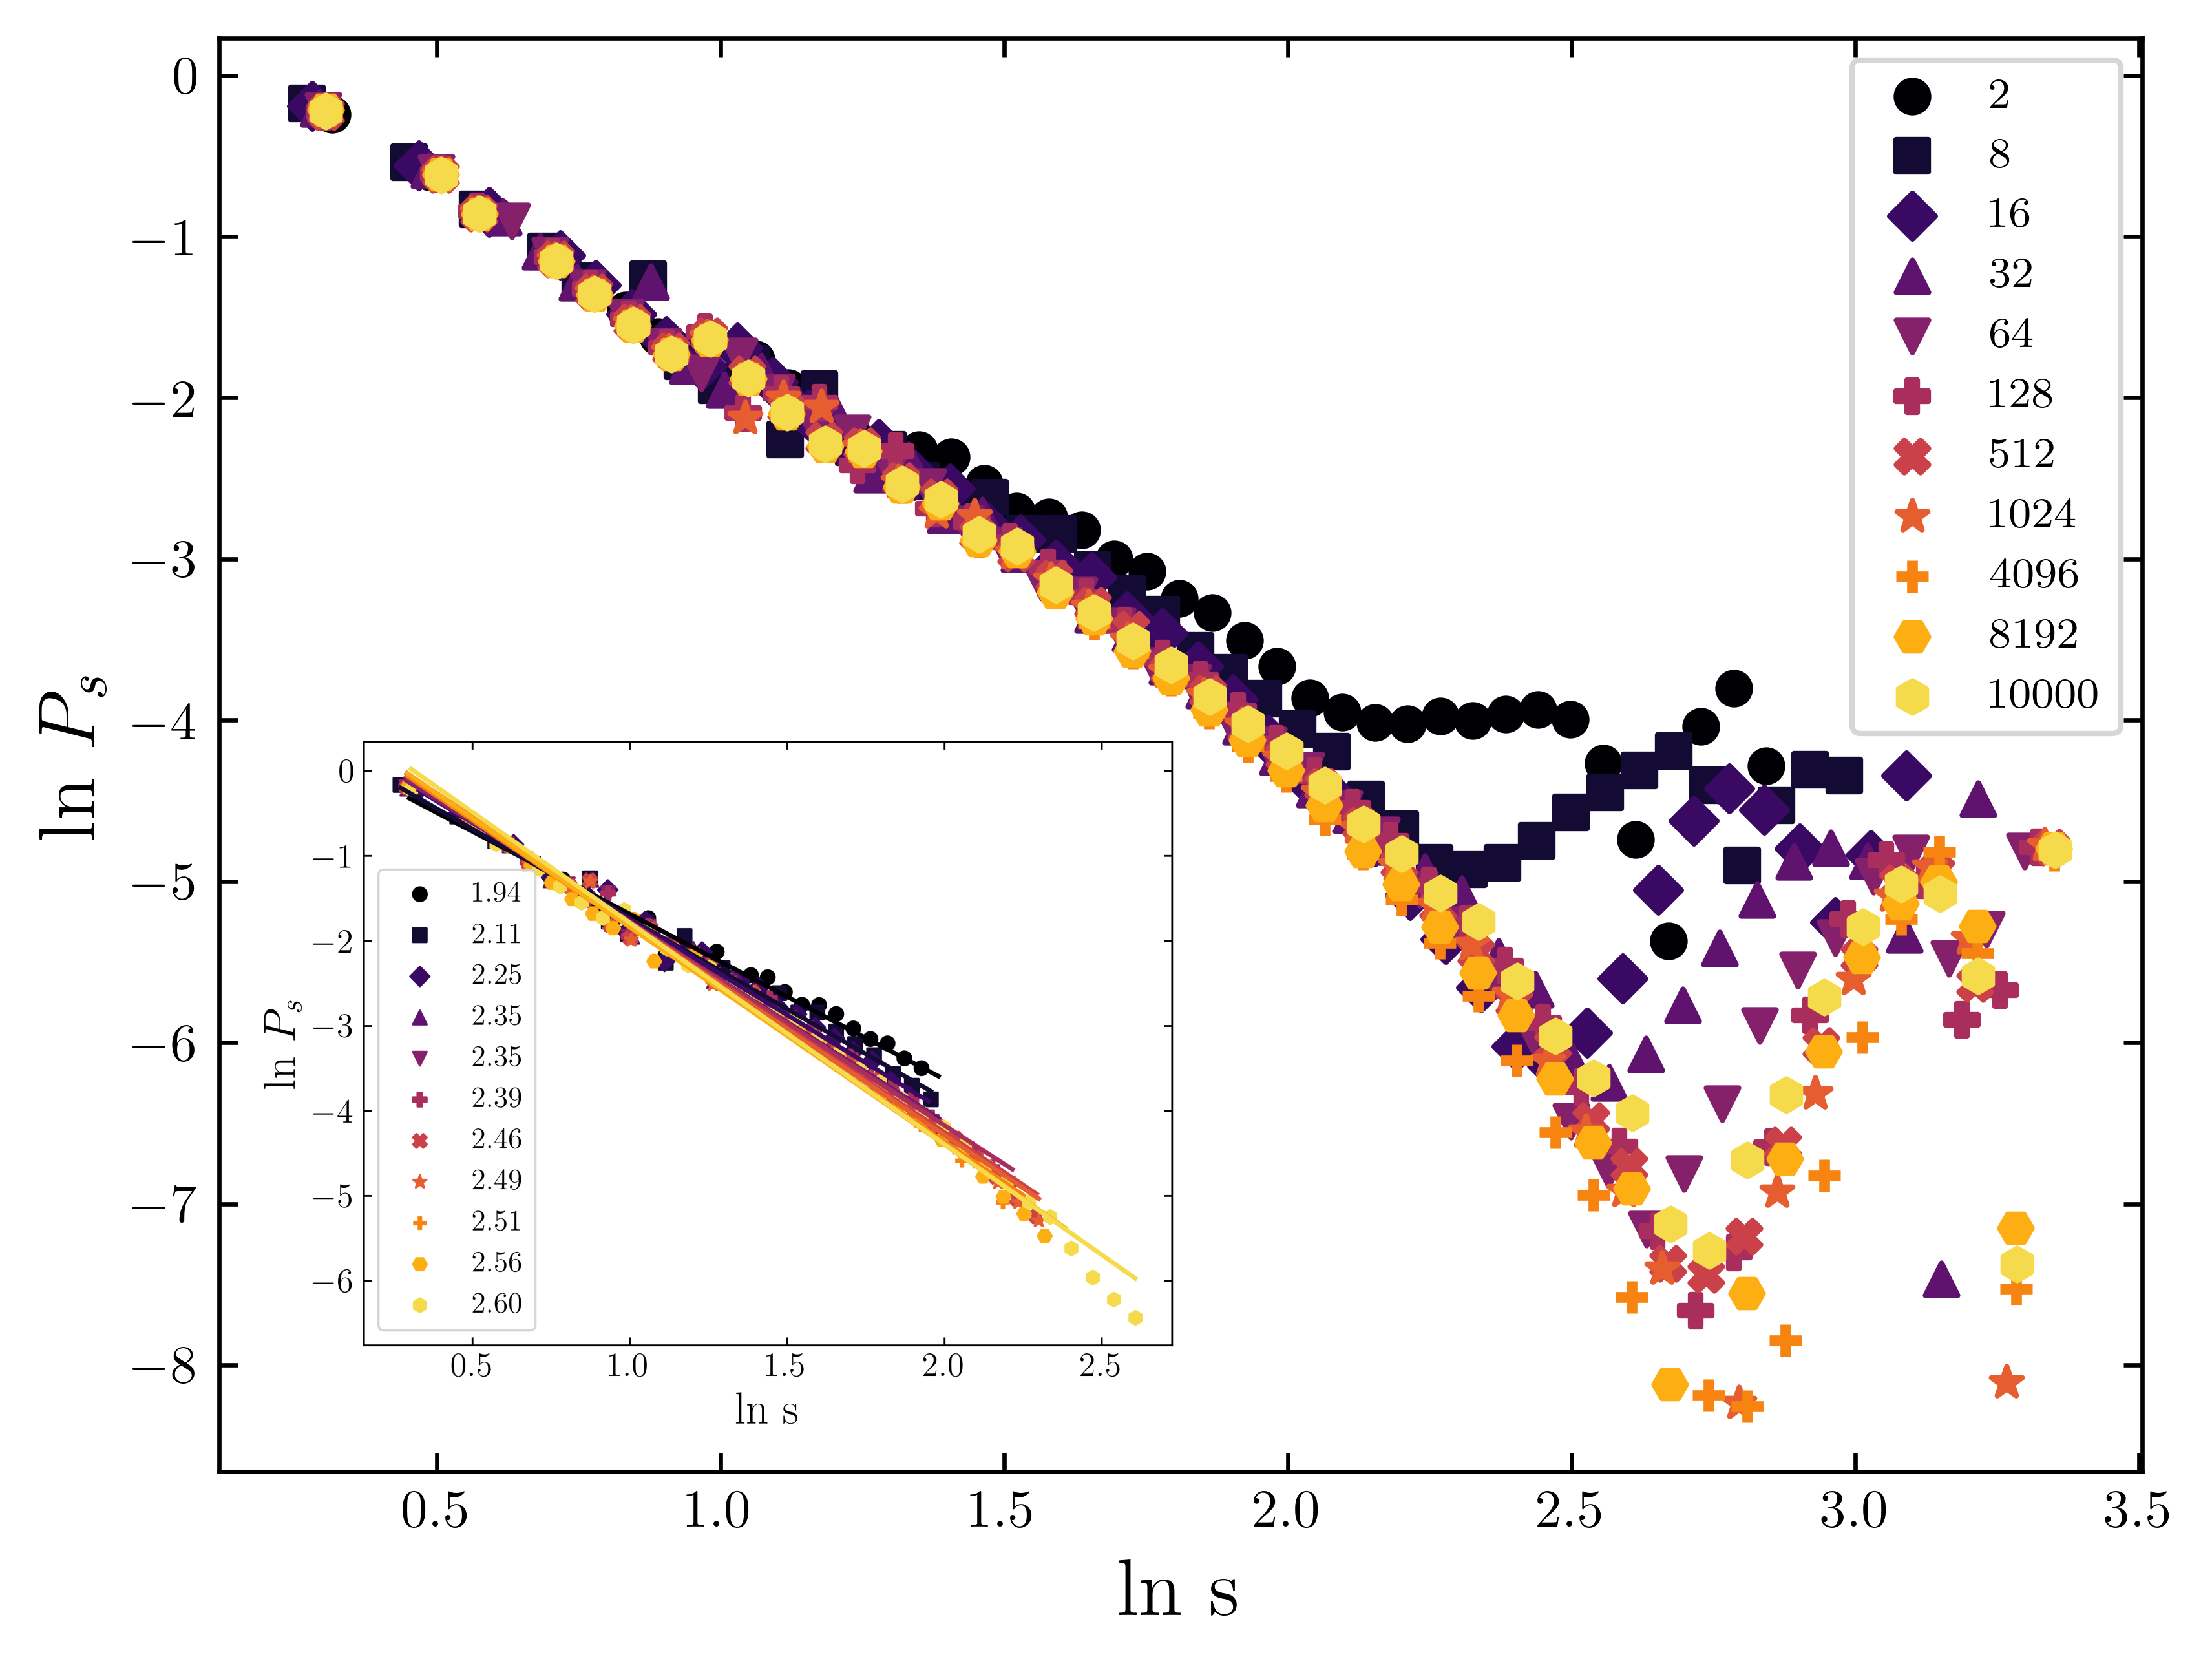
\includegraphics[width=\textwidth]{figures/ava.png}

        \caption{Distribuição das avalanches de ruptura em função do seu tamanho para diferentes valores de \(T_{s}\).
        Podemos observar um comportamento em lei de potencia com expoentes $\gamma$ bem definidos para todos valores do 
        parâmetro. Os expoentes variam de -1.94 a -2.60.} 

        \label{R7}

    \end{figure}

\section{Conclusões}

    Neste estudo, demonstramos a capacidade de um modelo baseado em Agregação Limitada por Difusão (DLA) com difusão 
    superficial para simular a formação de fibrilas de colágeno, resultando em agregados com características morfológicas 
    semelhantes às das fibrilas reais. O parâmetro \(T_{s}\) mostrou-se cruciail para definir várias propriedades das 
    fibrilas, como comprimento, densidade e diâmetro, que tendem a variar de maneira inversamente proporcional a \(T_{s}\). 
    Observou-se uma relação linear entre a massa das fibrilas e a distância até as pontas, além de uma variação na dimensão 
    fractal da seção central, que aumenta com \(T_{s}\), variando de 1.71 a 1.93.

    A resistência máxima à tensão das fibrilas aumenta com \(T_{s}\), alcançando um limite de 44,1 MPa, e a tensão crítica 
    suportada apresenta uma correlação exponencial com a densidade das fibrilas. O processo de ruptura revelou avalanches 
    de ruptura com leis de potência definidas, cujos expoentes variam de -1.94 a -2.60, indicando que, embora as avalanches 
    sejam independentes do tamanho do sistema, elas são influenciadas pela compactação da fibrila.

    Essas descobertas sugerem que as fibrilas geradas pelo modelo apresentam uma tensão máxima suportada que aumenta com a 
    densidade e com \(T_{s}\). Fibrilas mais resistentes tendem a ter uma dimensão fractal mais próxima da dimensão 
    euclidiana de objetos bidimensionais e exibem valores mais elevados no expoente das leis de potência. Além disso, muitas 
    das propriedades analisadas tendem a saturar, indicando que simulações realizadas com \(T_{s} = 512\) são suficientes para 
    observar os valores máximos de interesse, otimizando o uso de recursos computacionais.






\bibliographystyle{plain} % Set the bibliography style
\bibliography{ref} % Include your .bib file (without the .bib extension)


    
\end{document}
